\documentclass[pdf, 9pt]{beamer}

\mode<presentation>
{
  \usetheme{Warsaw}
  % or ...%

  \setbeamercovered{transparent}
  % or whatever (possibly just delete it)
}

% packages to be used
\usepackage[english]{babel}
\usepackage{times}
\usepackage[T1]{fontenc}
\usepackage[]{subfigure}
\usepackage[]{graphicx}
\usepackage{siunitx}
\usepackage{tikz}
\usepackage{amsmath}
\usepackage{multirow}

%
% some settings
%
\setbeamertemplate{itemize/enumerate body begin}{\normalsize}
\setbeamertemplate{itemize/enumerate subbody begin}{\small}

%
% define new comands
%
\newcommand {\framedgraphics}[2] {
    \begin{frame}{#1}
        \begin{center}
            \includegraphics[width=\textwidth,height=0.8\textheight,keepaspectratio]{#2}
        \end{center}
    \end{frame}
}

\newcommand\PlaceText[3]{%
\begin{tikzpicture}[remember picture,overlay]
\node[outer sep=0pt,inner sep=0pt,anchor=south west]
  at ([xshift=#1,yshift=-#2]current page.north west) {#3};
\end{tikzpicture}%
}

%
% Title, Author, Institution, etc
%
\title[PhD Defense]{PhD Defense}
\author[Viktor Khristenko]{V. Khristenko\inst{1}}
\institute[The University of Iowa]
{
  \inst{1}
  Department of Physics, The University of Iowa
}
\date[Defense 2017]
{PhD Defense, 2017}
\subject{Experimental High Energy Physics}

%
% Table of contents - outline
%
% Delete this, if you do not want the table of contents to pop up at
% the beginning of each subsection:
\AtBeginSection[]
{
  \begin{frame}<beamer>{Outline}
    \tableofcontents[currentsection]
  \end{frame}
}

%
% Begin the presentation
%
\begin{document}
\begin{frame}
  \titlepage
\end{frame}

\begin{frame}{Outline}
  \tableofcontents
  % You might wish to add the option [pausesections]
\end{frame}

%
% Introduction part
%
\section*{Where we stand}
  \begin{frame}{Where we stand}
    \begin{itemize}
      \item 5 years at The University of Iowa as PhD Student
        \begin{itemize}
            \item Test Beams at Fermilab and CERN
        \end{itemize}
      \item 3 years at CERN working on Compact Muon Solenoid Experiment
        \begin{itemize}
          \item CMS 2015 Achievement Award
          \item HCAL Operations Deputy Coordinator
          \item HCAL DQM Group Lead.
        \end{itemize}
      \item Received CERN IT Fellowship to work as Big Data Engineer.
    \end{itemize}
  \end{frame}

%
% Higgs Section
%
\section{Search for Standard Model Higgs Boson decaying to 2 muons with CMS}
  \begin{frame}{Introduction: Standard Model}
    \begin{columns}[T]
      \begin{column}{0.6\textwidth}
        \begin{itemize}
          \item Standard Model - Quantum Field Theory
          \item Incorporates Electromagnetic, Weak, Strong forces
          \item Force Carriers (Bosons) and matter constituents (Fermions)
          \item Bosons: gluons, vector bosons.
          \item Fermions: 6 quarks and 6 leptons.
        \end{itemize}
      \end{column}
      \begin{column}{0.4\textwidth}
        \begin{center}
          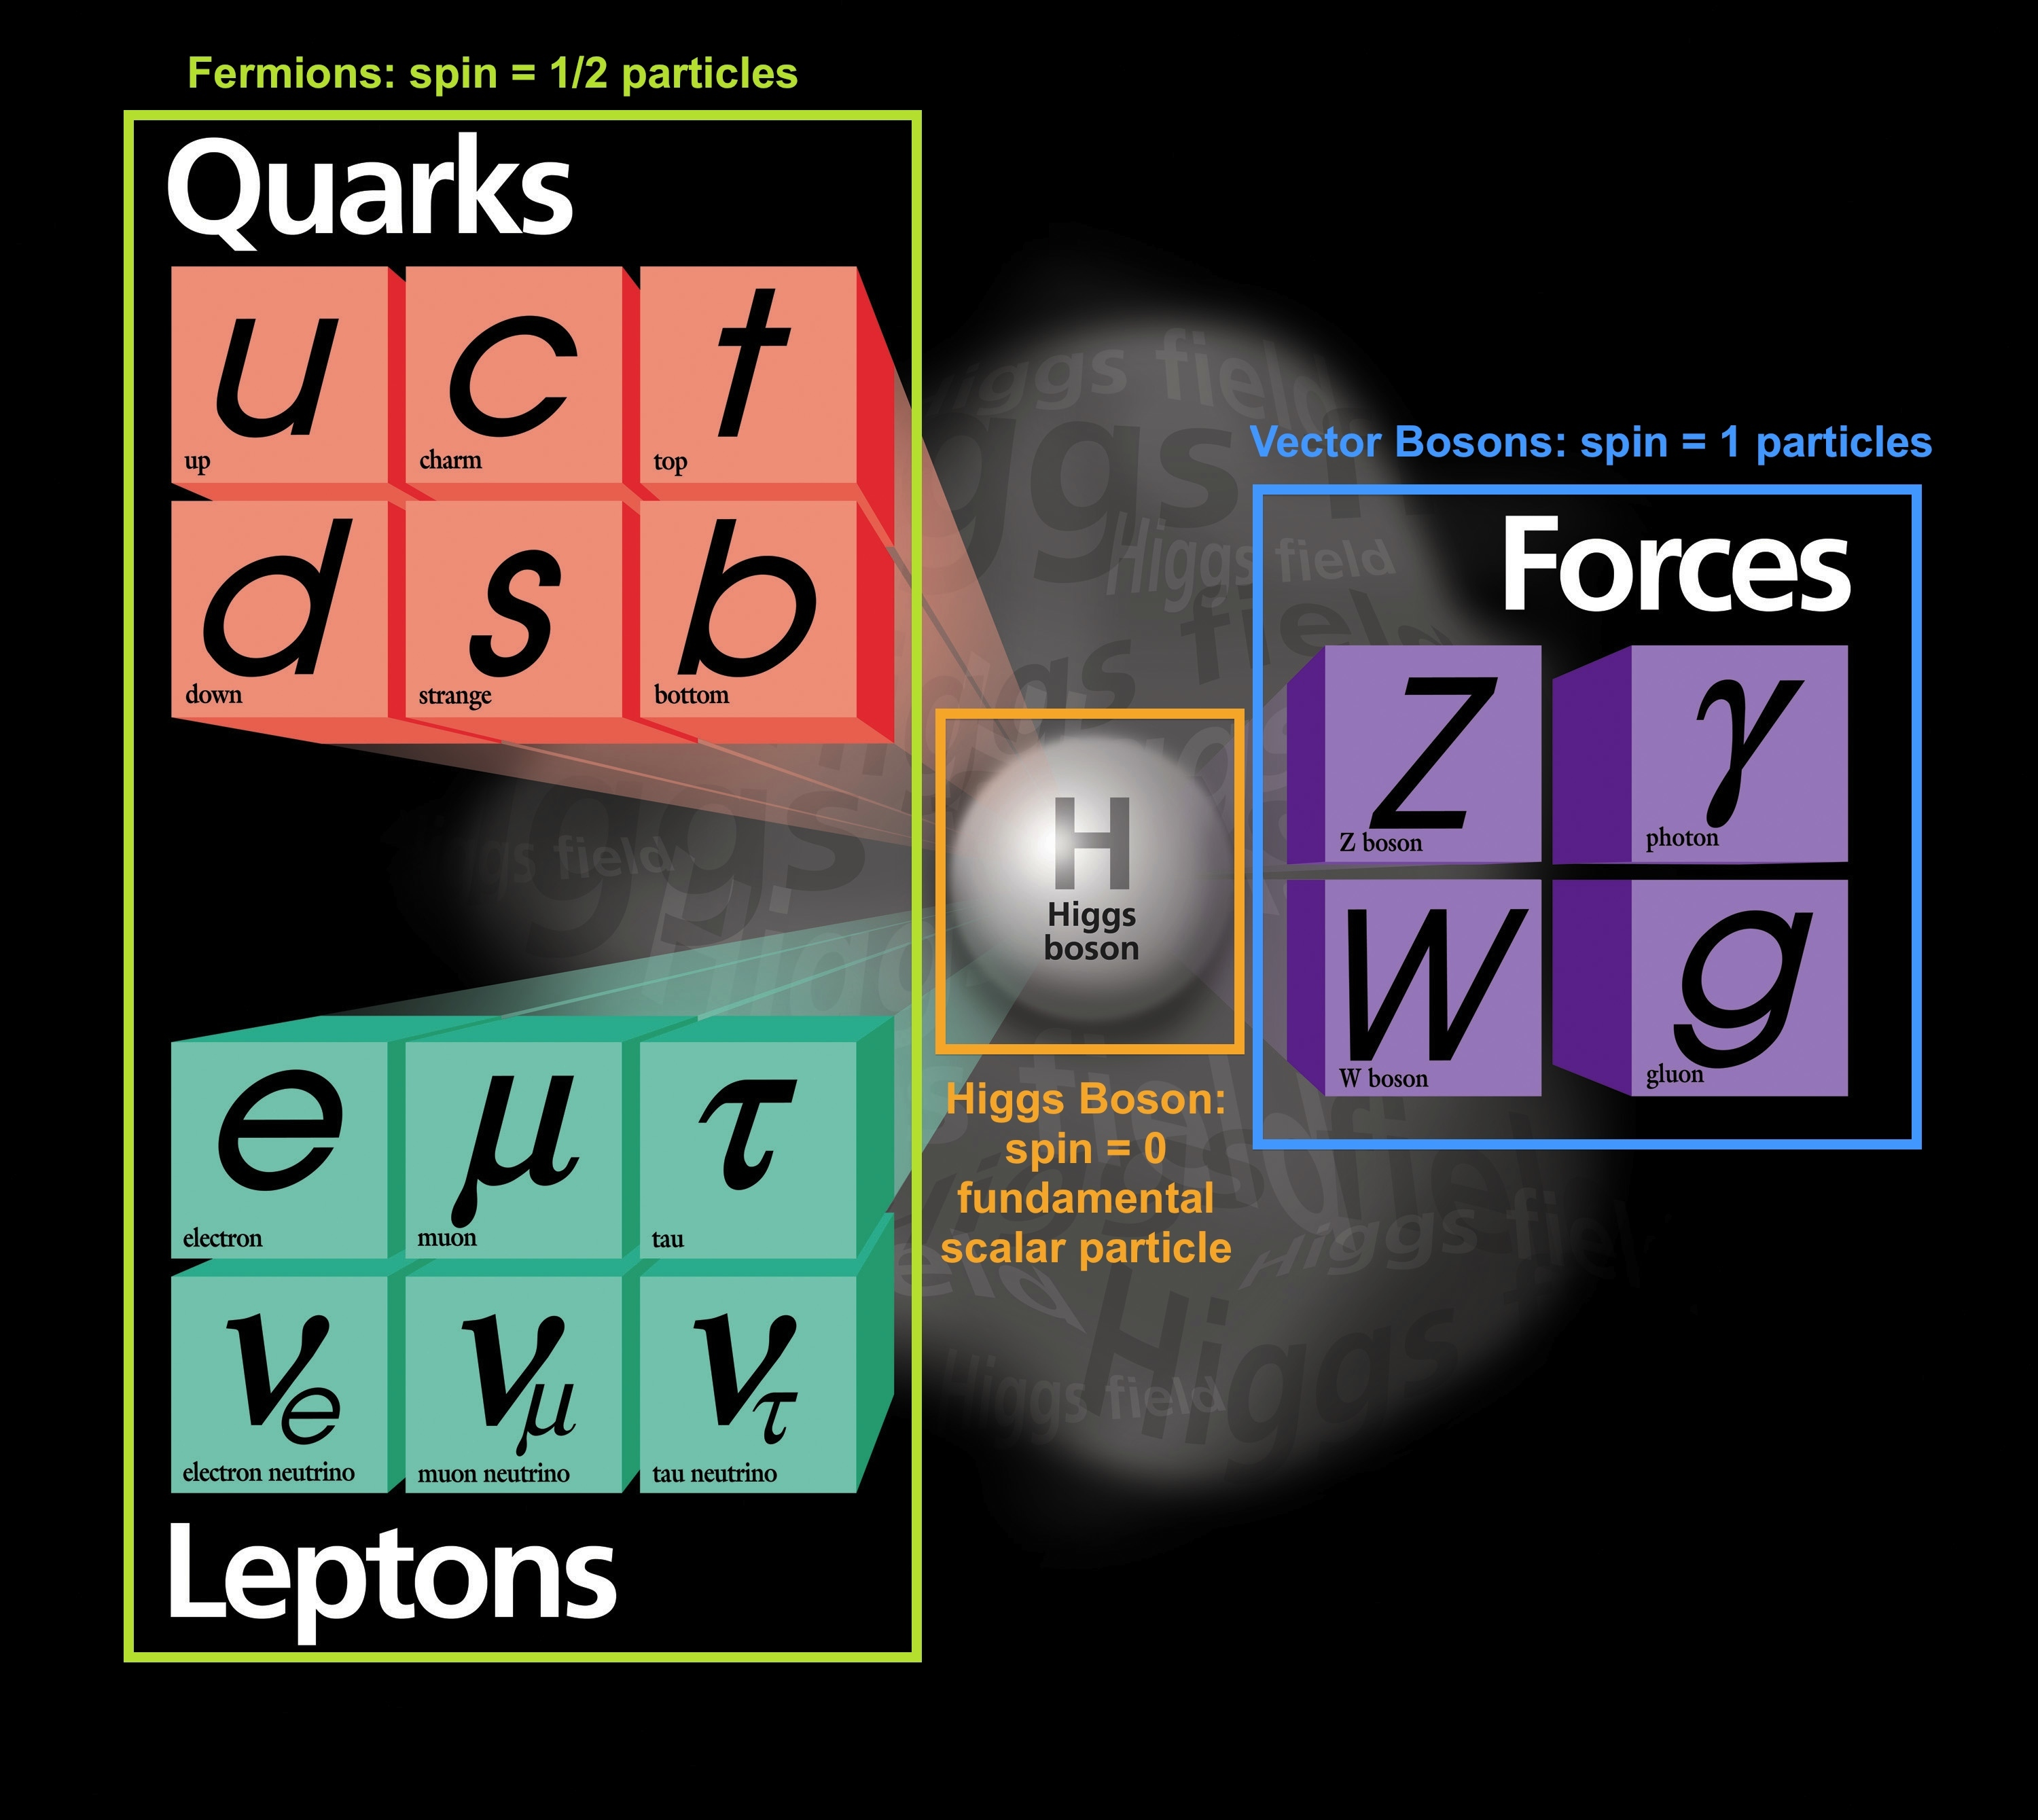
\includegraphics[width=0.99\textwidth, height=0.45\textheight]{figs/sm/sm.jpeg}
        \end{center}
      \end{column}
    \end{columns}
    \begin{block}{Remark}
      \begin{itemize}
        \item What is Higgs Boson and where does it fit into SM?!
        \item Why searching Higgs Boson decaying into 2 muons?!
      \end{itemize}
    \end{block}
  \end{frame}

  % \begin{frame}{Introduction: Standard Model}
  %   \begin{itemize}
  %     \item Local Gauage Invariant
  %   \end{itemize}
  % \end{frame}

  \begin{frame}{Introduction: Standard Model U(1)}
    \textbf{-} Start with a Lagrangian for a free fermion:\\
    \begin{equation}
      \label{eq:higgs_introduction_diracLagrangian}
      \mathcal{L} = \bar{\psi}i\gamma^{\mu}\partial_{\mu}\psi - m\bar{\psi}\psi
    \end{equation}
    \textbf{-} 2 types of transformations:\\\vspace{-0.3cm}
    \begin{subequations}\label{grp}
    \begin{align}
      Global:&\quad \psi \rightarrow e^{i\theta}\psi\\
      Local:&\quad \psi \rightarrow e^{i\theta(x)}\psi\label{eq:higgs_introduction_localgauge}
    \end{align}
    \end{subequations}
    \textbf{-} Local Transformation does not hold $\rightarrow$ introduce a vector field $A^{\mu}$:
    \begin{subequations}\label{eq:higgs_introduction_qedgauge}
    \begin{align}
      A^{\mu}& \rightarrow A^{\mu} - \frac{1}{q}\partial^{\mu}\theta(x)\label{eq:higgs_introduction_photonfieldu1}\\
      D^{\mu}& = \partial^{\mu} + iqA^{\mu}\label{eq:higgs_introduction_covariantderivative}
    \end{align}
    \end{subequations}
    \textbf{-} We obtain the Quantum Electrodynamics Lagrangian (almost):\\
    \begin{equation}
      \label{eq:higgs_introduction_diracLagrangianwithvectormass}
      \mathcal{L} = \bar{\psi}i\gamma^{\mu}D_{\mu}\psi - m\bar{\psi}\psi - \frac{1}{4}F^{\mu\nu}F_{\mu\nu} + m_{A}^{2}A^{\mu}A_{\mu}
    \end{equation}
    \textbf{-} \alert{For $m_{A}^{2}A^{\mu}A_{\mu}$ is not local gauge invariant $\rightarrow$ $m_{A} = 0$}\\
    \textbf{-} \alert{$m\bar{\psi}\psi$ is U(1) local gauge invariant}
  \end{frame}

  \begin{frame}{Introduction: Standard Model - SU(2) and SU(2)$_L$}
    \textbf{-} Consider 2 fermionic fields and define a doublet:\\\vspace{-0.2cm}
    \begin{equation}
      \Psi = (\psi_1, \psi_2)
    \end{equation}
    \textbf{-} Require a free Lagrangian to be invariant under Transformations:\\\vspace{-0.3cm}
    \begin{subequations}\label{eq:higgs_introduction_gaugesu2}
    \begin{align}
      Global:&\quad \Psi \rightarrow e^{i\boldsymbol{\theta} \cdot \boldsymbol{\sigma}}\Psi\\
      Local:&\quad \Psi \rightarrow e^{i\boldsymbol{\theta(x)} \cdot \boldsymbol\sigma}\Psi\label{eq:higgs_introduction_localgaugesu2}
    \end{align}
    \end{subequations}
    \textbf{-} Will introduce 3 new massless vector fields.\\
    \textbf{-} Define Chiral Projections for a Dirac-field (4-component):\\\vspace{-0.7cm}
    \begin{subequations}\label{eq:higgs_introduction_chiralprojections}
    \begin{align}
      \psi_L& = \frac{1}{2}(1 - \gamma^{5})\psi\\
      \psi_R& = \frac{1}{2}(1 + \gamma^{5})\psi\\
      m\bar{\psi}\psi& = m \bar{\psi_L}\psi_R + m \bar{\psi_R}\psi_L
    \end{align}
    \end{subequations}
    \textbf{-} \alert{Standard Model Electroweak theory imposes gauge invariance only for left-handed fermions! $\rightarrow$ SU(2)$_L$}
  \end{frame}

  \begin{frame}{Introduction: Standard Model - Problems and Solutions}
    \begin{itemize}
      \item SU(2)$_L$ $\times$ U(1) $\rightarrow$ 3 Massless Vector fields - contrary to observation
      \item $\psi_L$ transforms according to SU(2)$_L$ $\times$ U(1), $\psi_R$ according to U(1) $\rightarrow$ Fermions are massless - contrary to observation
    \end{itemize}
    \begin{block}{Remark}
      Solution: Higgs Mechanism - a new field living in SU(2)$_L$ $\times$ U(1) and a particular choice of the potential term. Upon Spontaneous Symmetry Breaking - masses for gauge bosons are generated!
    \end{block}
    \begin{block}{Quote}
      S. Coleman: ''In general, there is no reason why an invariance of the Hamiltonian of a quantum-mechanical system should also be an invariance of the ground state of the system.''
    \end{block}
  \end{frame}

  \begin{frame}{Introduction: Standard Model - Higgs Mechanism}
    \textbf{-} Adding an SU(2) doublet field - 4 degrees of freedom:\\
    \begin{align}\Phi& =\begin{bmatrix} \phi_1 + i\phi_2 \\ \phi_3 + i\phi_4 \end{bmatrix}\end{align}
    \textbf{-} With a Potential Term:\\\vspace{-0.3cm}
    \begin{subequations}
    \begin{align}
      V(\Phi)& = \mu^2\Phi^{\dagger}\Phi + \lambda(\Phi^{\dagger}\Phi)^2\\
      \mu^2& < 0
    %   \mathcal{L}& = \mathcal{L}_{fermion} + \mathcal{L}_{new}\\
    % & = \bar{\Psi}i\gamma^{\mu}D_{\mu}\Psi + (D^{\mu}\Phi)^{\dagger}D_{\mu}\Phi - \mu^2\Phi^{\dagger}\Phi - \lambda(\Phi^{\   dagger}\Phi)^2
    \end{align}
    \end{subequations}
    \textbf{-} With a Lagrangian:\\\vspace{-0.3cm}
    \begin{subequations}
    \begin{align}
      \mathcal{L}& = \bar{\Psi}i\gamma^{\mu}D_{\mu}\Psi + (D^{\mu}\Phi)^{\dagger}D_{\mu}\Phi - \mu^2\Phi^{\dagger}\Phi - \lambda(\Phi^{\dagger}\Phi)^2
    \end{align}
    \end{subequations}
    \textbf{-} With a Yukawa coupling to fermions
    \begin{subequations}
    \begin{align}
      m\bar{\psi}\psi& \rightarrow y [\bar{\psi_L}\phi\psi_R + \bar{\psi_R}\bar{\phi}\psi_L]\\
      & \rightarrow y[\begin{bmatrix} \bar{\psi_1}, \bar{\psi_2} \end{bmatrix}_L\begin{bmatrix} \phi_1 + i\phi_2 \\ \phi_3 + i\phi_4 \end{bmatrix} \psi_R + \bar{\psi}_R\begin{bmatrix} \phi_1^{\dagger} - i\phi_2^{\dagger}, \phi_3^{\dagger} - i\phi_4^{\dagger} \end{bmatrix}\begin{bmatrix} \psi_1 \\ \psi_2 \end{bmatrix}_L]
    \end{align}
    \end{subequations}
  \end{frame}

  \begin{frame}{Introduction: Higgs Mechanism}
    \textbf{-} Perturb the, $\Phi$-field, SU(2) $\times$ U(1) doublet around the minimum:\\\vspace{-0.5cm}
    \begin{align}
      \Phi& =\begin{bmatrix} \phi_1 + i\phi_2 \\ \phi_3 + i\phi_4 \end{bmatrix}
      \rightarrow \begin{bmatrix} \phi_1 + i\phi_2 \\ H + \nu + i\phi_4 \end{bmatrix},
      \nu = \sqrt{-\frac{\mu^2}{\lambda}}
    \end{align}
    \textbf{-} Expand Lagrangian and select the Unitary Gauge\\
    \textbf{-} $\phi_1$, $\phi_2$, $\phi_3$ components will be absorved (upon choosing the Unitary Gauge) into mass terms for 3 vector bosons by expanding the kinetic term:\\\vspace{-0.5cm}
    \begin{subequations}
    \begin{align}
      \mathcal{L}_{kinetic}& = (D^{\mu}\Phi)^{\dagger}D_{\mu}\Phi
    \end{align}
    \end{subequations}
    \textbf{-} Fermion mass and Coupling to Higgs Field will come from:\\\vspace{-0.5cm}
    \begin{subequations}
    \begin{align}
      m\bar{\psi}\psi& \rightarrow y [\bar{\psi_L}\phi\psi_R + \bar{\psi_R}\bar{\phi}\psi_L]\\
      & \rightarrow y[\begin{bmatrix} \bar{\psi_1}, \bar{\psi_2} \end{bmatrix}_L\begin{bmatrix} 0 \\ H + \nu \end{bmatrix} \psi_R + \bar{\psi}_R\begin{bmatrix} 0, H + \nu \end{bmatrix}\begin{bmatrix} \psi_1 \\ \psi_2 \end{bmatrix}_L]\\
      & \rightarrow y\sqrt{-\frac{\mu^2}{2\lambda}}\bar{\psi}_{Dirac}\psi_{Dirac} + \frac{y}{\sqrt{2}}H\bar\psi_{Dirac}\psi_{Dirac}
    \end{align}
    \end{subequations}
  \end{frame}

  \begin{frame}{Introduction: Summary}
      \textbf{-} Original phenomenological Lagrangian possesses local gauge invariance!\\
      \textbf{-} Spontaneous Symmetry Breaking, \alert{by definition}, is the change of the ground state to another ground state under certain transformation - local SU(2)$_L$ $\times$ U(1) for SM!\\
      \textbf{-} Real Higgs Field!\\
      \textbf{-} Mass for the fermions:\\\vspace{-0.4cm}
      \begin{subequations}
      \begin{align}
        y\sqrt{-\frac{\mu^2}{2\lambda}}\bar{\psi}_{Dirac}\psi_{Dirac} \rightarrow m = \frac{y\nu}{\sqrt{2}}
      \end{align}
      \end{subequations}
      \textbf{-} Yukawa Coupling of Higgs to Fermions\\
      \textbf{-} At 125 GeV Higgs boson mass, Branching Fraction is 0.00022\\
      \begin{subequations}
      \begin{align}
      \mathcal{B}(H \rightarrow \mu\mu)& = \frac{\Gamma(H \rightarrow \mu\mu)}{\sum \Gamma(H \rightarrow \dots)}
      \end{align}
      \end{subequations}
  \end{frame}

  % \begin{frame}{Introduction: Standard Model - SU(2)$_L$ and Problems}
  %   \textbf{-} local SU(2) invariance $\rightarrow$ 3 massless vector bosons
  %   \textbf{-} Experiment, however, shows that W$^{+/-}$ and Z$^{0}$ are massive
  %   \textbf{-}
  % \end{frame}

{ % all template changes are local to this group.
    \setbeamertemplate{navigation symbols}{}
    \begin{frame}[plain]
        \begin{tikzpicture}[remember picture,overlay]
            \node[at=(current page.center)] {
                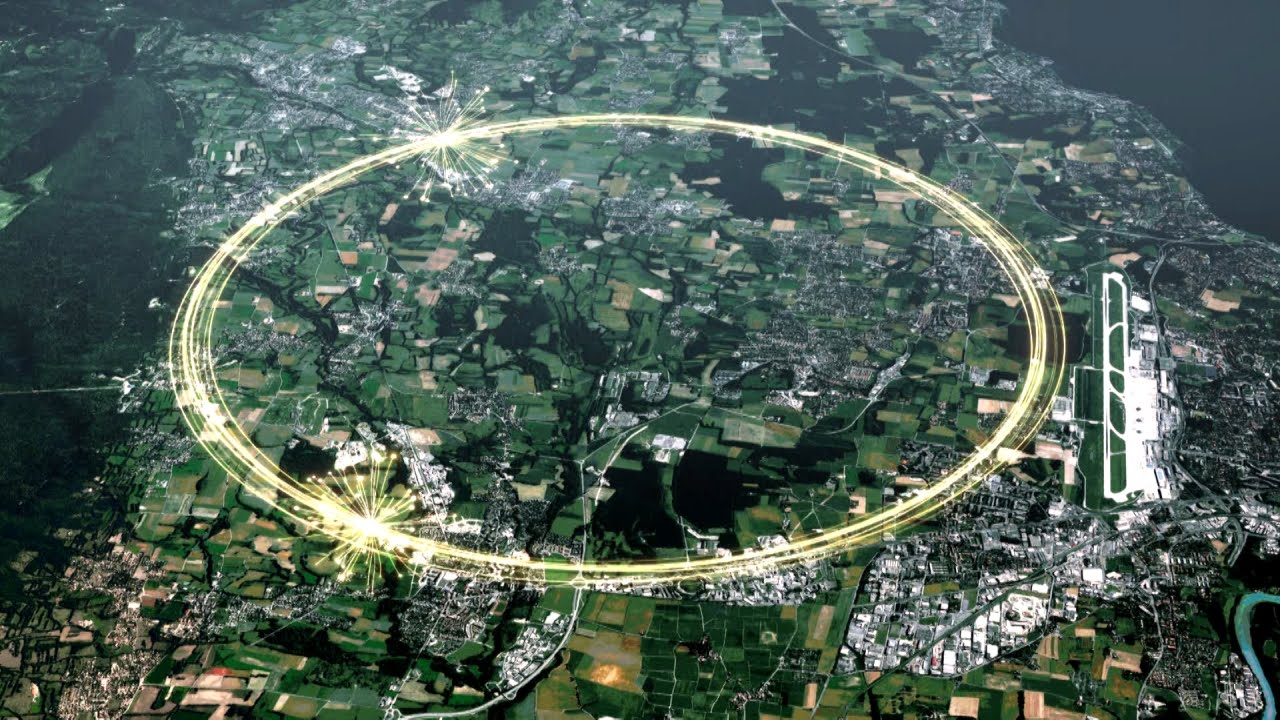
\includegraphics[width=\paperwidth]{figs/lhc/maxresdefault.jpg}
            };
        \end{tikzpicture}
     \end{frame}
}

  \begin{frame}{Large Hadron Collider}
    \begin{columns}[T]
      \begin{column}{0.6\textwidth}
        \begin{itemize}
          \item LHC - Accelerating Complex
          \item Accelerates/Collides pp, Pb-p, Pb-Pb
          \item Current maximum momentum per beam is 6.5TeV/c ($\sqrt{s}=13TeV$) for proton beam
          \item ``Data Factory'' one of its kind
            \begin{itemize}
              \item Even without recording collisions
            \end{itemize}
        \end{itemize}
      \end{column}
      \begin{column}{0.4\textwidth}
        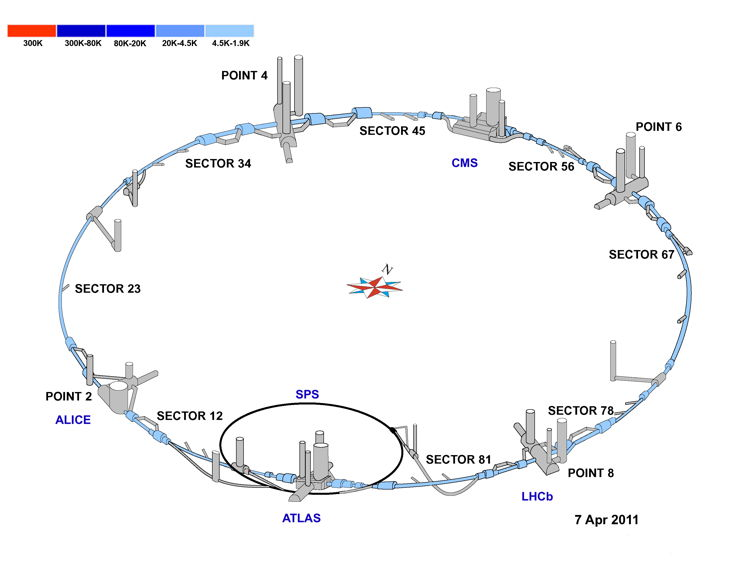
\includegraphics[width=0.99\textwidth, height=0.55\textheight, keepaspectratio]{figs/lhc/LHC_Fig1.jpg}
      \end{column}
    \end{columns}
  \end{frame}

  { % all template changes are local to this group.
    \setbeamertemplate{navigation symbols}{}
    \begin{frame}[plain]
        \begin{tikzpicture}[remember picture,overlay]
            \node[at=(current page.center)] {
                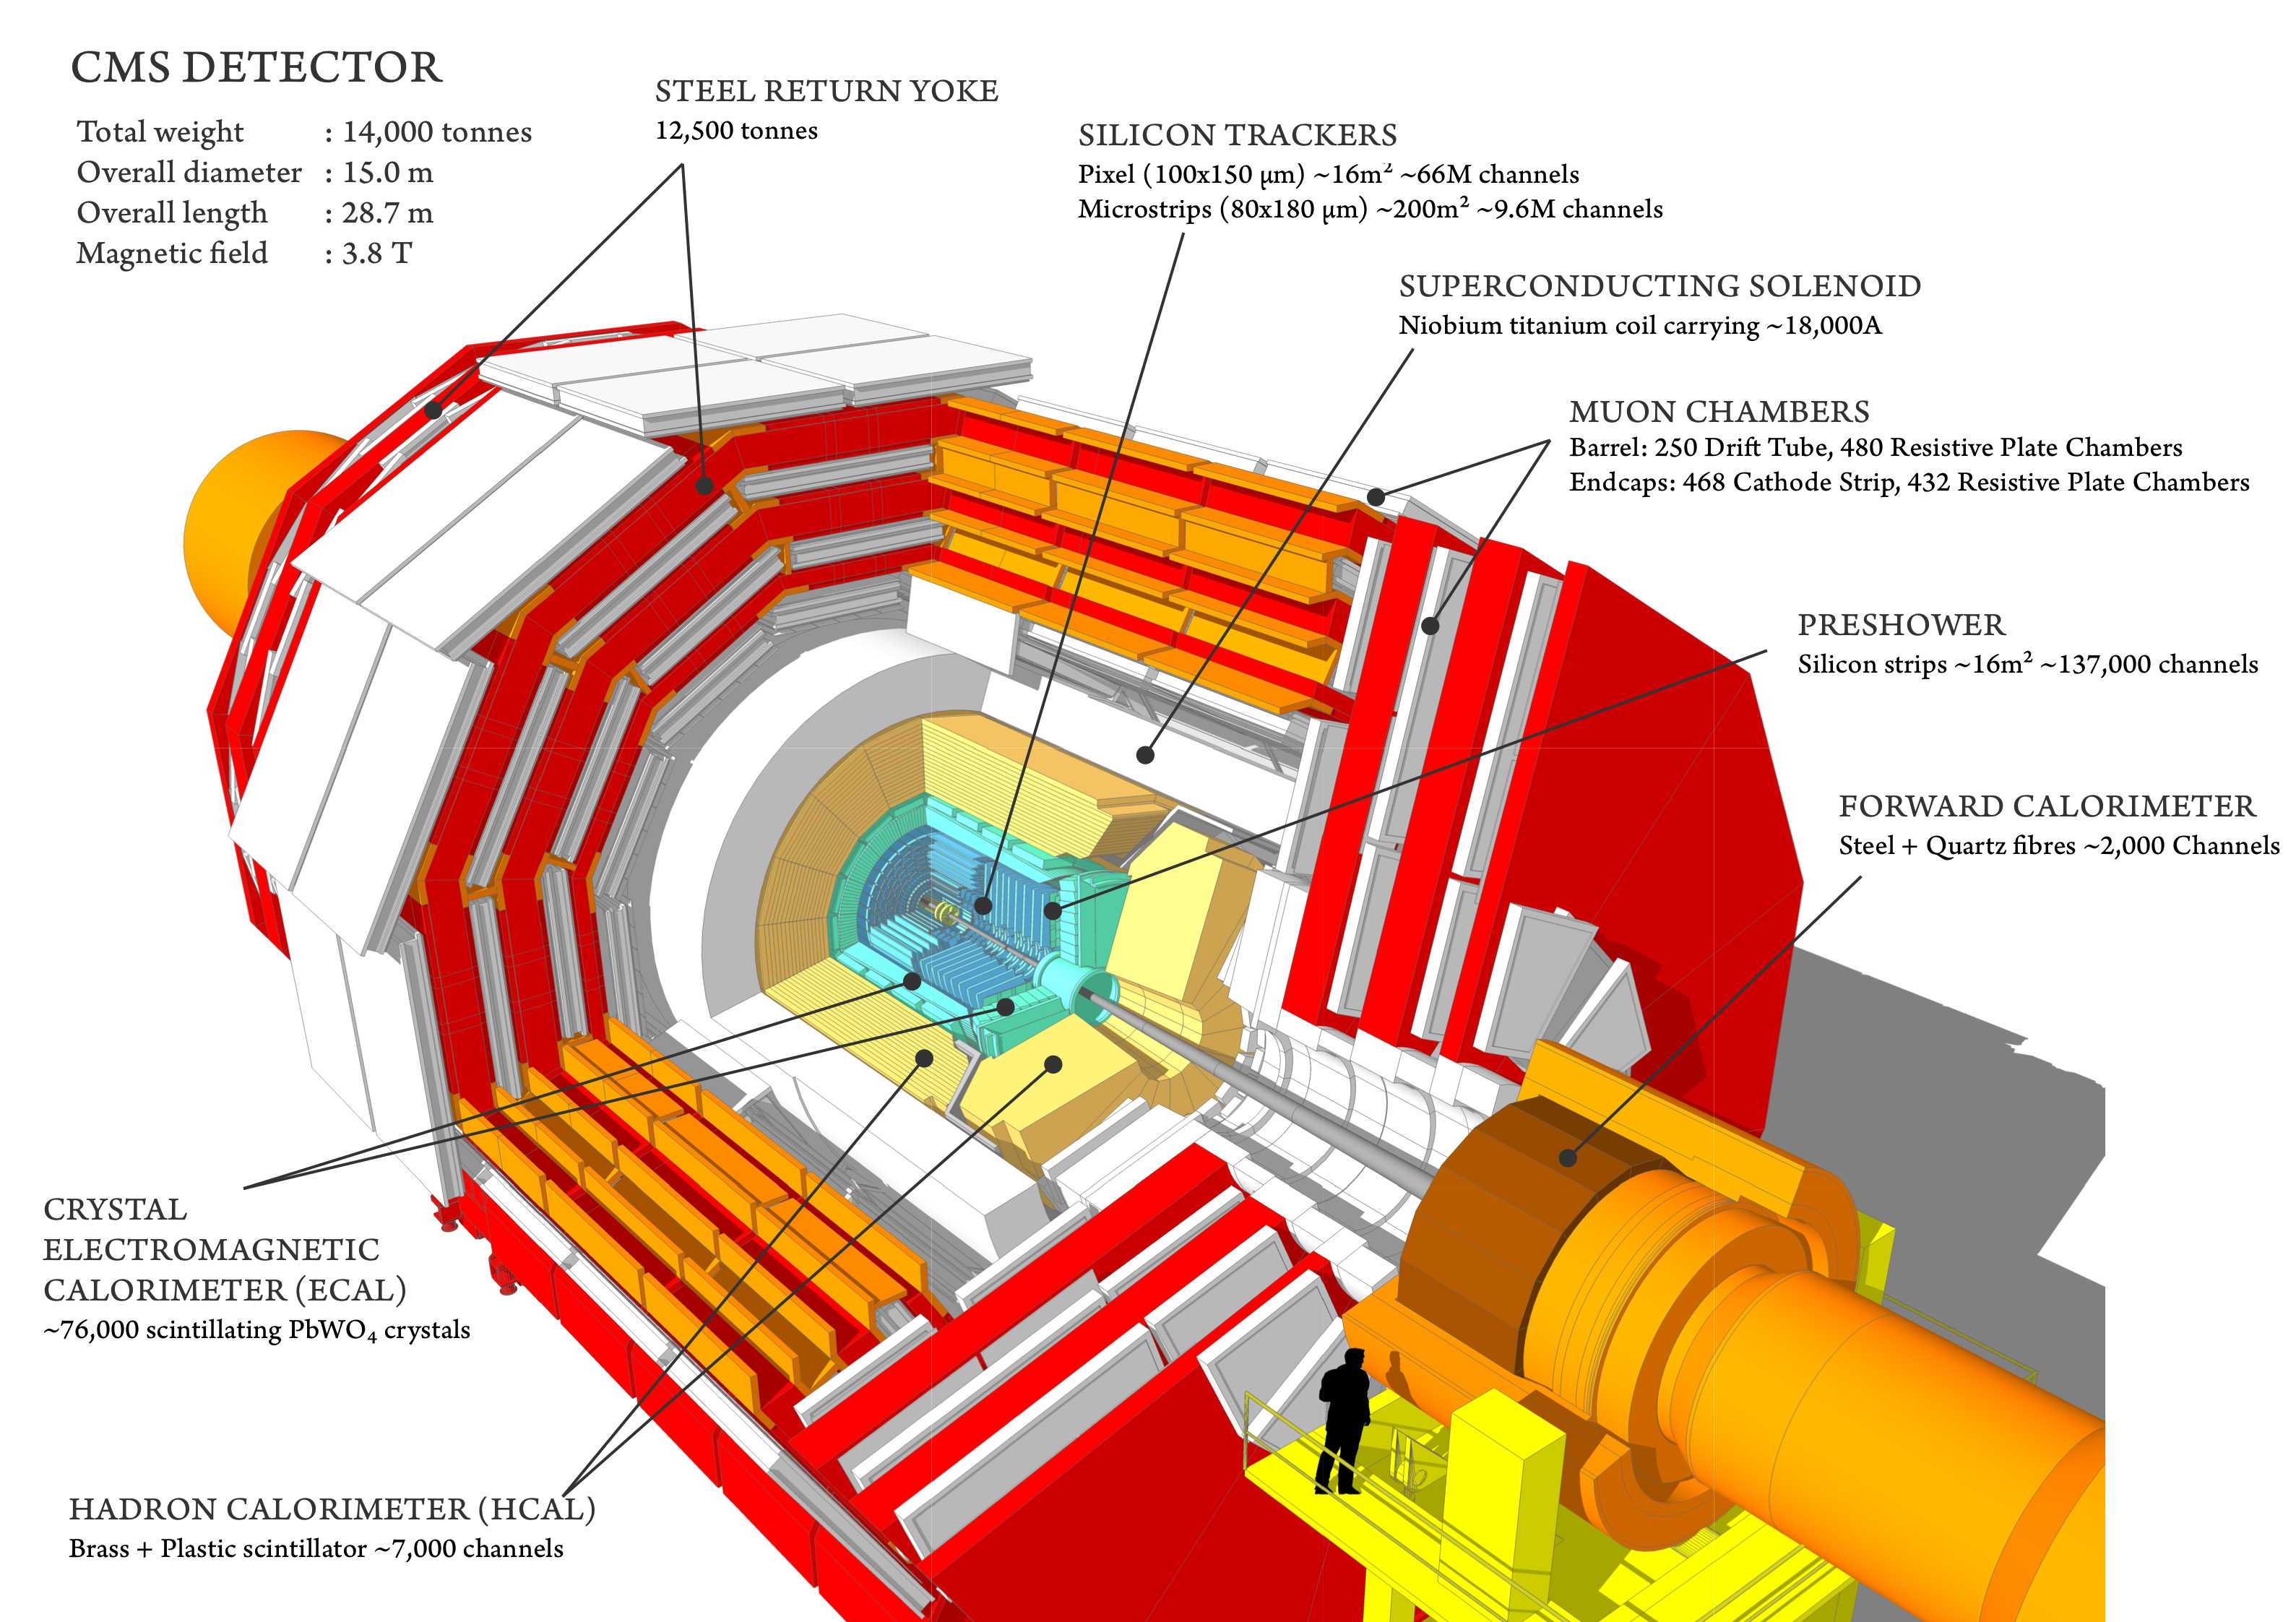
\includegraphics[width=\paperwidth]{figs/cms/cms_120918_03.png}
            };
        \end{tikzpicture}
     \end{frame}
}

  { % all template changes are local to this group.
    \setbeamertemplate{navigation symbols}{}
    \begin{frame}[plain]
        \begin{tikzpicture}[remember picture,overlay]
            \node[at=(current page.center)] {
                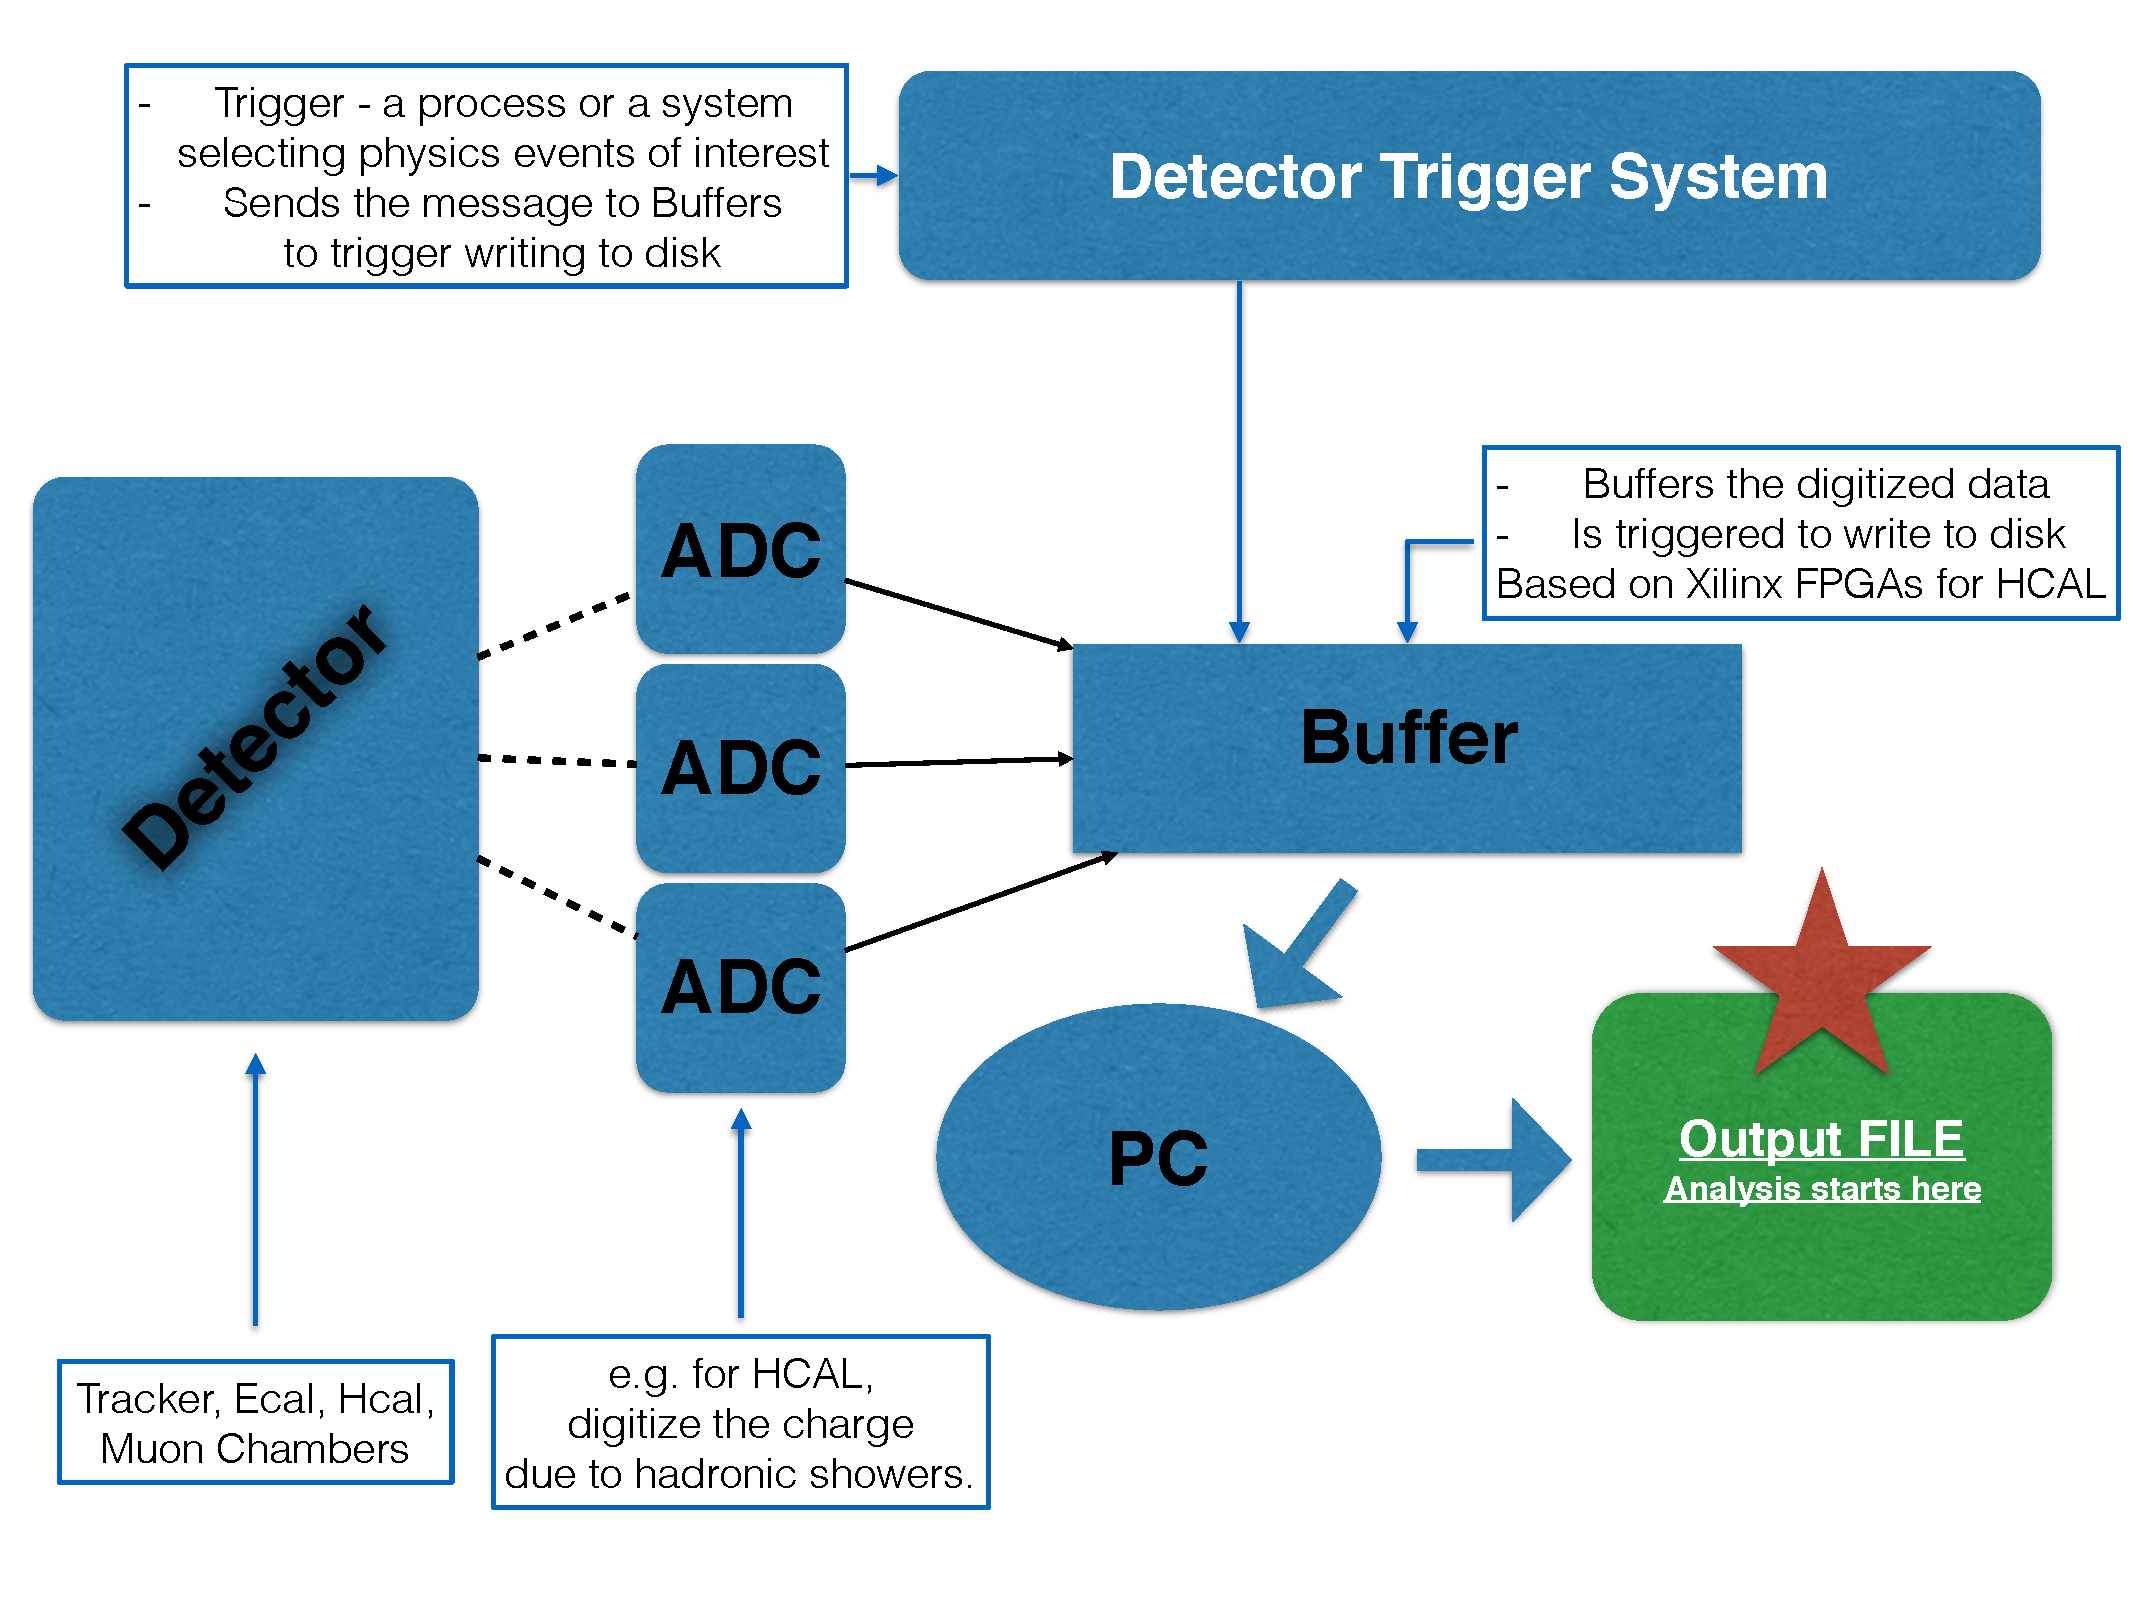
\includegraphics[width=\paperwidth]{figs/cms/cms_dataflow_simple.pdf}
            };
        \end{tikzpicture}
     \end{frame}
}

  % \begin{frame}{Compact Muon Solenoid}
  %   \begin{center}
  %     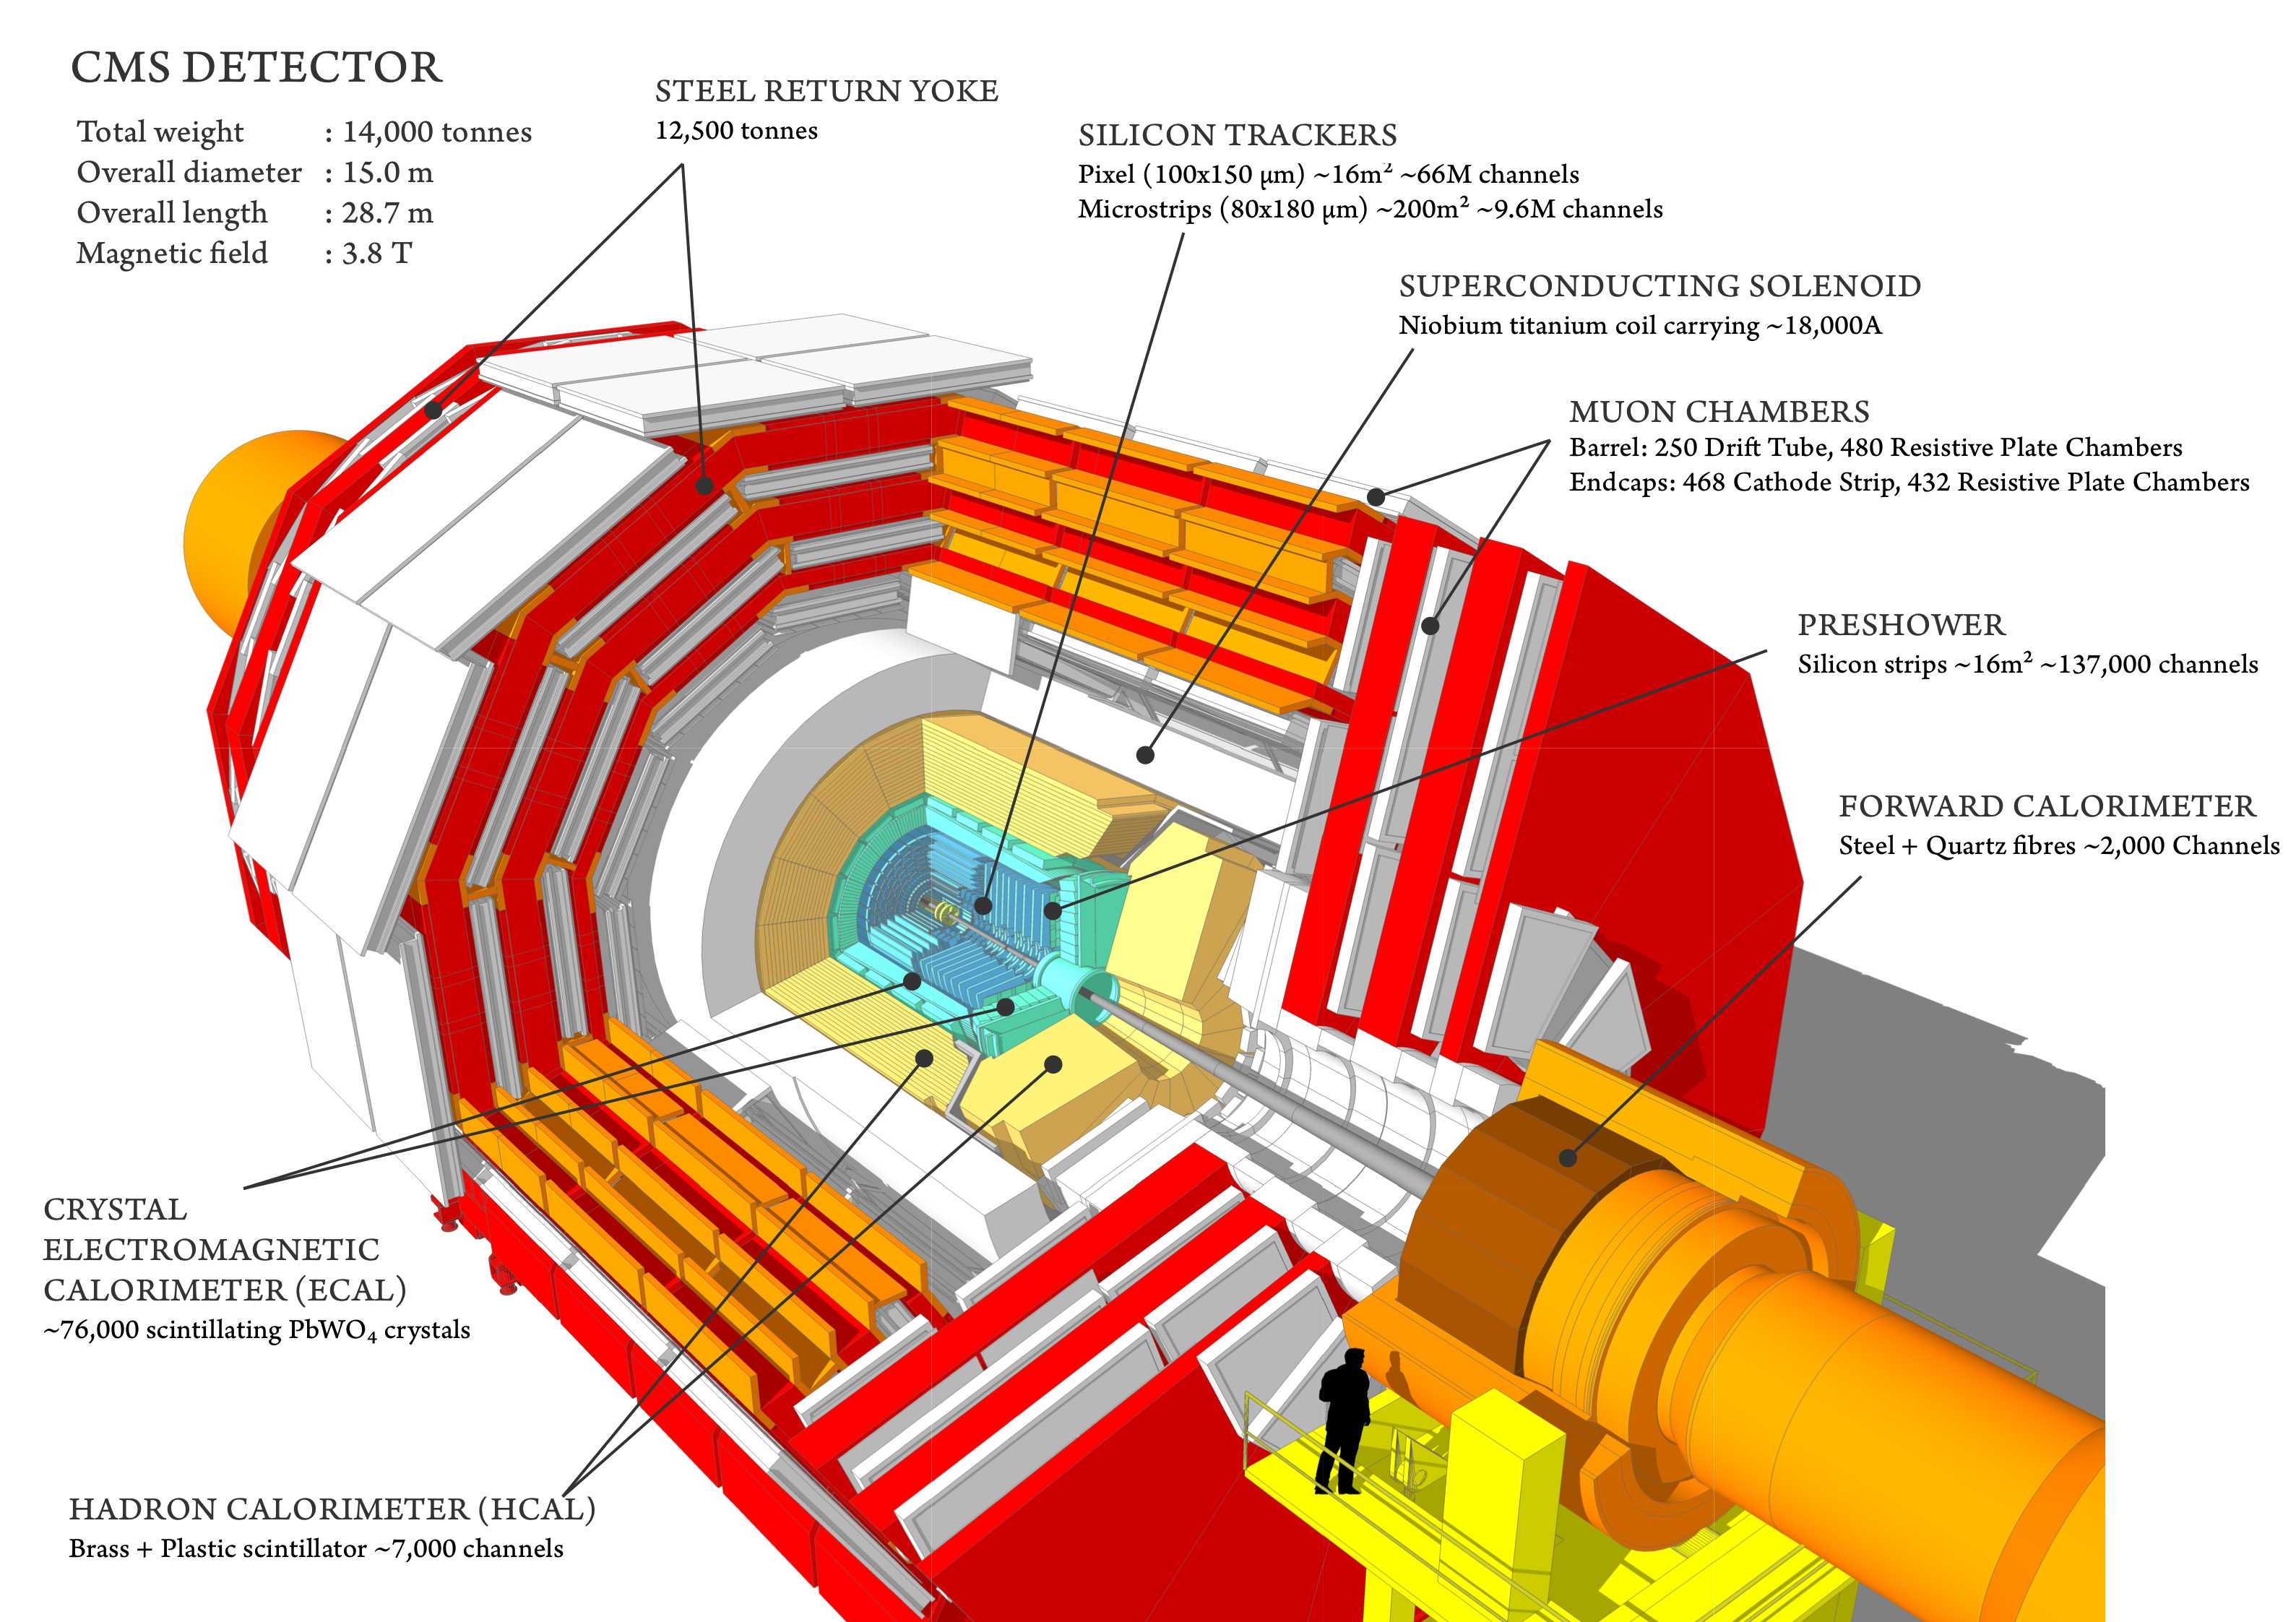
\includegraphics[width=0.99\textwidth, height=0.9\textheight]{figs/cms/cms_120918_03.png}
  %   \end{center}
  % \end{frame}

  \begin{frame}{SM Higgs Search at CMS in Run I}
    \begin{columns}[T]
      \begin{column}{0.7\textwidth}
        \begin{itemize}
          \item Run I proton-proton collsions at $\sqrt{s}=7 TeV (L = 5 fb^{-1})$ and $\sqrt{s}=8 TeV (L = 19.7 fb^{-1})$
          \item CMS made observations of Higgs Boson
            \begin{itemize}
              \item $H \rightarrow \gamma\gamma$
              \item $H \rightarrow ZZ \rightarrow 4l$
              \item $H \rightarrow \tau\tau$
              \item \alert{no observation for $H \rightarrow \mu\mu$}
            \end{itemize}
          \item \alert{$1.1\sigma$ excess in significance} for mass $125GeV$ was observed - compatible with statistical fluctuation
          \item $95\%$ Confidence Level (CL) exclusion limits were set on $125GeV$ Higgs Production Cross-Section.
            \begin{itemize}
              \item for $7TeV \rightarrow \sigma = 12.8 \times SM$(Exp.) and \alert{$\sigma = 19.0 \times SM$(Obs.)}
              \item for $8TeV \rightarrow \sigma = 5.6 \times SM$(Exp.) and \alert{$\sigma = 6.9 \times SM$(Obs.)}
            \end{itemize}
        \end{itemize}
      \end{column}
      \begin{column}{0.3\textwidth}
        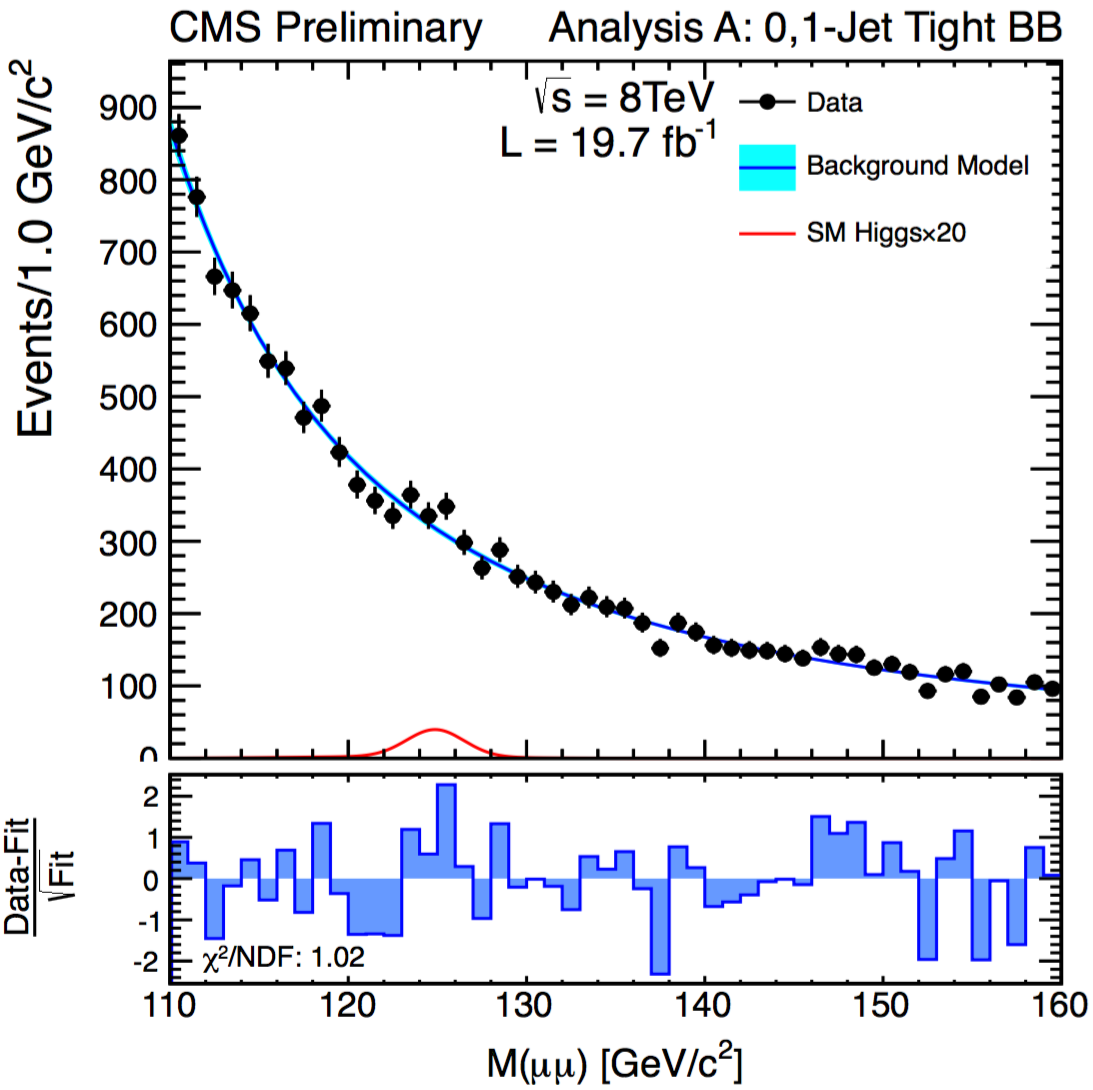
\includegraphics[width=0.99\textwidth, height=0.28\textheight]{figs/higgs/run1/HIGpas_fit_01JetTightBB.png}\\
        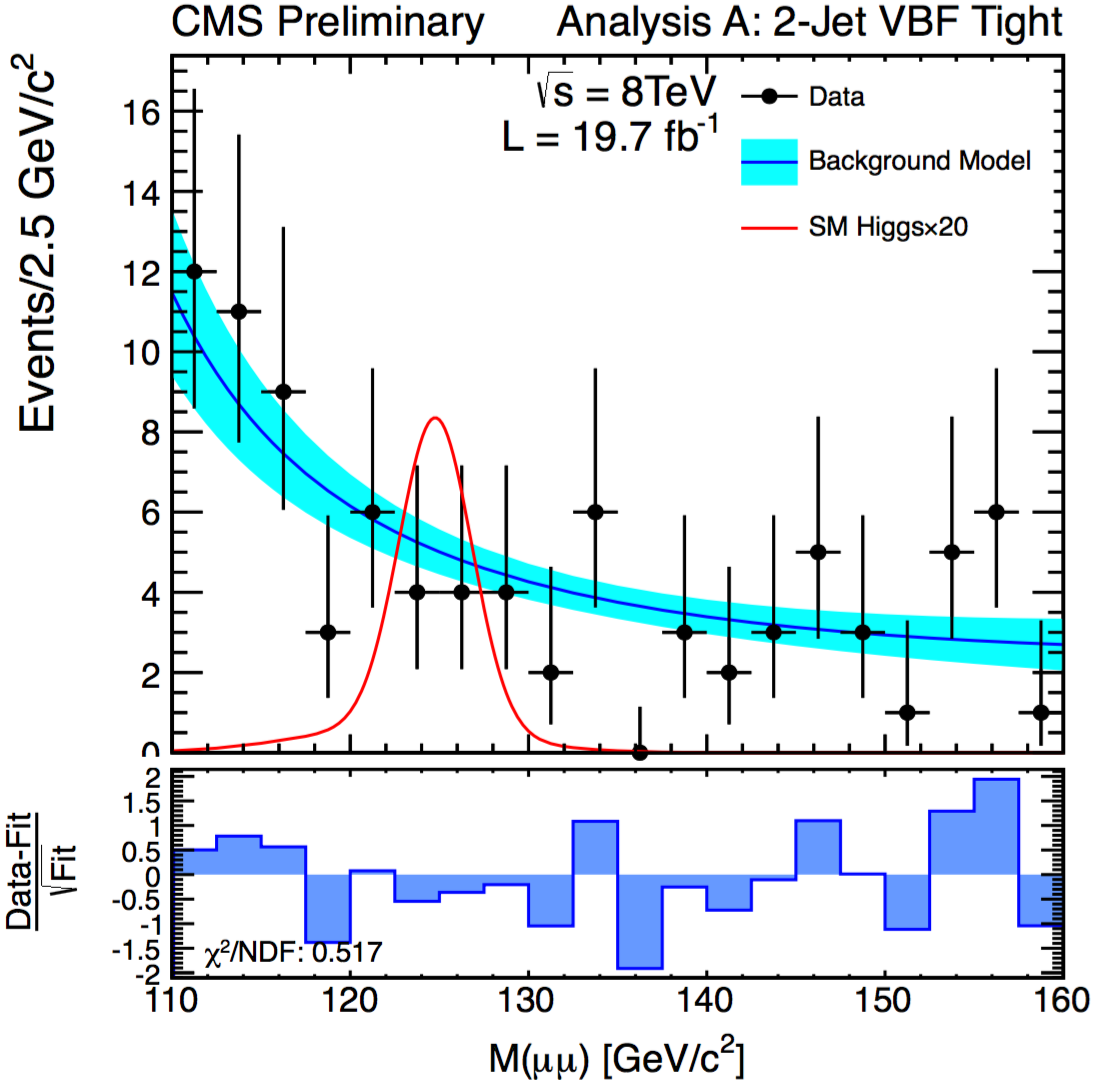
\includegraphics[width=0.99\textwidth, height=0.28\textheight]{figs/higgs/run1/HIGpas_fit_VBFTight.png}\\
        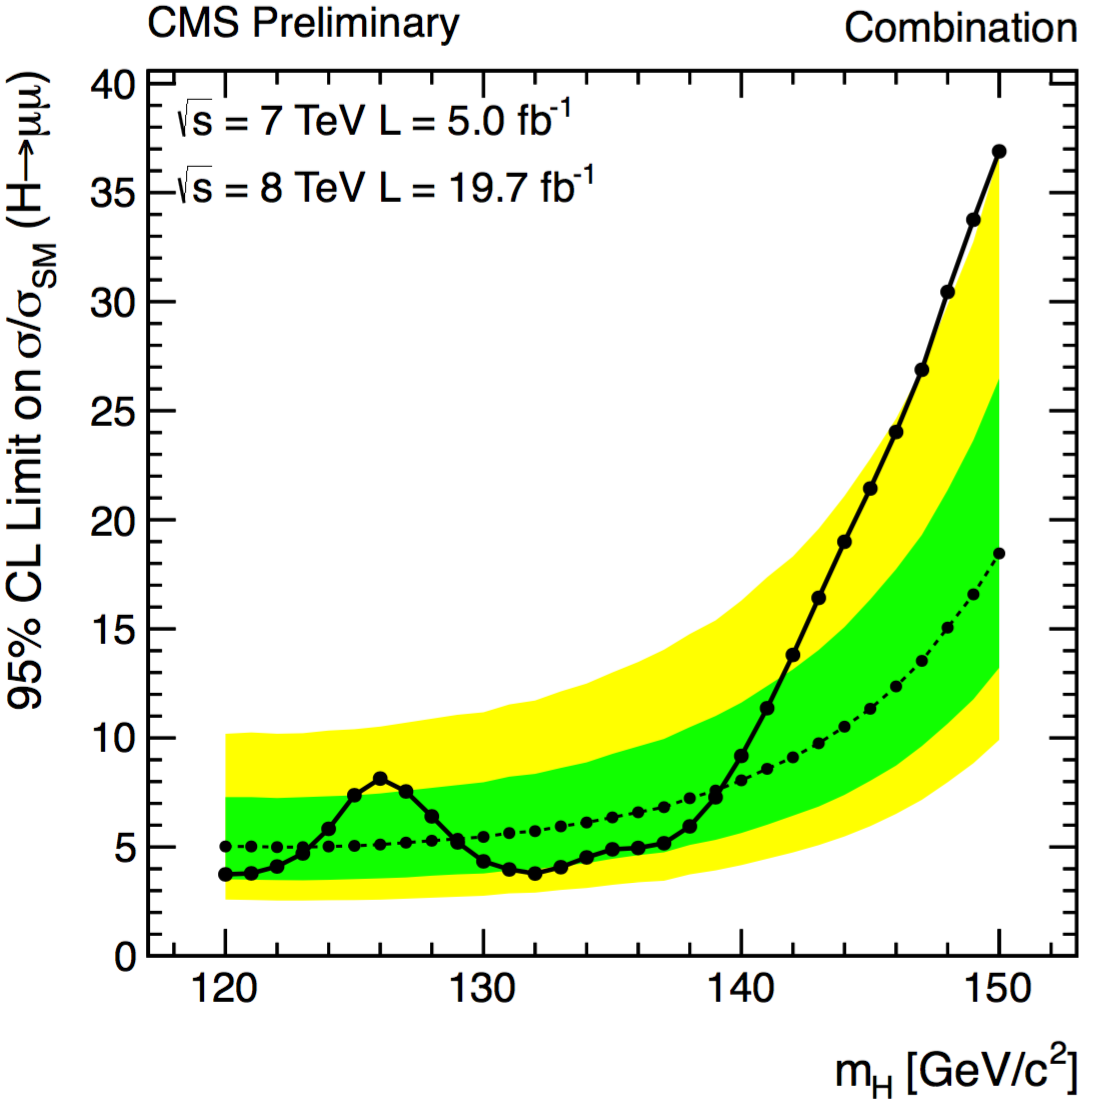
\includegraphics[width=0.99\textwidth, height=0.28\textheight]{figs/higgs/run1/HIGpas_limit_Combination.png}
      \end{column}
    \end{columns}
  \end{frame}

  \begin{frame}{Problem Statement}
    \begin{block}{Remark}
      The primary objective of this work is to investigate the $\mu^{+} \mu^{-}$ Higgs decay mode with 35.9 fb$^-1$ of data collected in proton-proton collisions at $\sqrt{s}=13$ TeV by Compact Muon Solenoid (CMS) Experiment during the second operational phase of LHC (2016)
    \end{block}
  \end{frame}


  \begin{frame}{Analysis Workflow}
    \begin{itemize}
      \item \alert{Collect the data!}
      \item Data Preprocesssing/Skimming
        \begin{itemize}
          \item Apply basic selection criteria (e.g. at least 2 muons in event)
          \item Reduce the amount of data by orders of magnitude.
        \end{itemize}
      \item Event Selections
        \begin{itemize}
          \item Apply muon corrections
          \item Apply various selections
          \item Choose objects of interest
          \item Compare Data with MC simulations and establish the validity of simulated models.
            \begin{itemize}
              \item If matches - good, does not - why?! Other models\dots ?
            \end{itemize}
        \end{itemize}
      \item Event Categorization
        \begin{itemize}
          \item Grouping events by \#jets, $p_{t}^{\mu\mu}$, BDT score, \dots
        \end{itemize}
      \item Compute Systematics
      \item Statistical Analysis
          \begin{itemize}
            \item Build Signal/Background Models
            \item Extract the 95\% CL Exclusion Limits
          \end{itemize}
    \end{itemize}
  \end{frame}

  \begin{frame}{Datasets and Configuration: General}
    \begin{itemize}
      \item Data
        \begin{itemize}
          \item Use $36.9$ fb$^{-1}$ of data collected over 2016
          \item SingleMuon Primary Dataset
        \end{itemize}
      \item Monte Carlo
        \begin{itemize}
          \item Higgs Signal
            \begin{itemize}
              \item VBF, ggFuson, W$^{+/-}$H, Zh production processes
            \end{itemize}
          \item Backgrounds
            \begin{itemize}
              \item Drell-Yan + Jets
              \item $t\bar{t}$ + Jets
              \item \dots
            \end{itemize}
          \item PileUp reweighting for 69.2 mb
        \end{itemize}
    \end{itemize}
  \end{frame}

  \begin{frame}{Datasets and Configuration: Data}
    \begin{table}[htb]
    \caption{Datasets for proton-proton collisions recorded at $\sqrt{s}=13$~TeV by CMS at LHC in 2016.}
    \label{table:higgs_data_collisiondatasets}
    \begin{center}
        \begin{tabular}{ l  c}
            \hline
            Datasets & Int. Luminosity (fb$^{-1}$)\\
            \hline
            {/SingleMuon/Run2016B-03Feb2017\_ver2-v2/MINIAOD} & 5.788\\
            {/SingleMuon/Run2016C-03Feb2017-v1/MINIAOD} & 2.573\\
            {/SingleMuon/Run2016D-03Feb2017-v1/MINIAOD} & 4.248\\
            {/SingleMuon/Run2016E-03Feb2017-v1/MINIAOD} & 4.009\\
            {/SingleMuon/Run2016F-03Feb2017-v1/MINIAOD} & 3.102\\
            {/SingleMuon/Run2016G-03Feb2017-v1/MINIAOD} & 7.540\\
            {/SingleMuon/Run2016H-03Feb2017\_ver2(3)-v1/MINIAOD} & 8.606\\
            \hline
        \end{tabular}
    \end{center}
    \end{table}
  \end{frame}

  \begin{frame}{Datasets and Configuration: SM Higgs Signal}
    \begin{table}[htb]
    \caption{Standard Model 125 GeV Higgs Boson Signal Datasets for 13 TeV. Dataset names for 120/130 GeV are omitted for brevity. Moriond 2017 conditions are used (omitted the conditions specification for brevity).}
    \label{table:higgs_data_signaldatasets}
    \begin{center}
        \begin{tabular}{ l  c}
            \hline
            Datasets & $\sigma$ (pb)\\
            \hline
            {/GluGlu\_HToMuMu\_M125\_13TeV\_powheg\_pythia8} & 48.58\\
            {/VBF\_HToMuMu\_M125\_13TeV\_powheg\_pythia8} & 3.782\\
            {/WMinusH\_HToMuMu\_M125\_13TeV\_powheg\_pythia8} & 0.5331\\
            {/WPlusH\_HToMuMu\_M125\_13TeV\_powheg\_pythia8} & 0.851\\
            {/ZH\_HToMuMu\_M125\_13TeV\_powheg\_pythia8} & 0.8839 \\
            \hline
        \end{tabular}
    \end{center}
\end{table}
  \end{frame}

  \begin{frame}{Datasets and Configuration: Backgrounds}
    \begin{table}[htb]
    \caption{Background Datasets. Moriond 2017 conditions have been used (omitted the conditions specification for brevity).}
    \label{table:higgs_data_backgrounddatasets}
    \begin{center}
        \begin{tabular}{ l  c}
            \hline
            Dataset & $\sigma$ (pb)\\
            \hline
            \small{/DYJetsToLL\_M-50\_TuneCUETP8M1\_13TeV-amcatnloFXFX-pythia8} & 5765\\
            \small{/ST\_tW\_top\_5f\_NoFullyHadronicDecays\_13TeV-powheg\_TuneCUETP8M1} & 35.85\\
            \small{/TTJets\_DiLept\_TuneCUETP8M1\_13TeV-madgraphMLM-pythia8} & 85.656\\
            \small{/WJetsToLNu\_TuneCUETP8M1\_13TeV-amcatnloFXFX-pythia8} & 61526.7\\
            \small{/WWTo2L2Nu\_13TeV-powheg-herwigpp} & 10.481\\
            \small{/WZTo3LNu\_TuneCUETP8M1\_13TeV-amcatnloFXFX-pythia8} & 4.712\\
            \hline
        \end{tabular}
    \end{center}
    \end{table}
  \end{frame}

  \begin{frame}{Event Selections}
    \begin{itemize}
      \item Primary Vertex
        \begin{itemize}
          \item at least 1 Primary Vertex with
          \item $|zPV| < 24$ - shift along the beam axis w.r.t. nominal CMS center
          \item $ndf > 4$ - degrees of freedom
        \end{itemize}
      \item HLT - HLT\_IsoMu24 or HLT\_IsoTkMu24 to fire
        \begin{itemize}
          \item \alert{Event must have at least 1 $\mu$ with $p_{t} \ge 24GeV$}
        \end{itemize}
      \item Jets
        \begin{itemize}
          \item $p_{t}>30$ GeV \&\& $|\eta|<4.7$ \&\& $\Delta R_{\mu} < 0.4$
        \end{itemize}
      \item Muons
        \begin{itemize}
          \item 2 oppositely charged muons
          \item Each Muon
            \begin{itemize}
              \item Rochester Muon Corrections
              \item Medium Muon Id
              \item $p_{t} > 10$ GeV \&\& $|\eta| < 2.4$ \&\& $I_{rel}^{PF} < 0.25$
            \end{itemize}
          \item At least 1 muon to match HLT
            \begin{itemize}
              \item $p_{t}>26$ GeV \&\& $|\eta|<2.4$ \&\& $\Delta R_{HLT} < 0.1$
            \end{itemize}
        \end{itemize}
      \item Passed basic event selections - identify this as the \alert{TopCategory} - combination of all.
    \end{itemize}
  \end{frame}

  \begin{frame}{Top Category: Mass Distribution}
    \begin{center}
    Dimuon Mass (m$_{\mu\mu}$) distribution with Rochester Muon Corrections:\\\vspace{0.1cm}
      % \begin{block}{Remark}
      %   Note the orders of magnitude difference between background and \alert{signal}!
      % \end{block}
      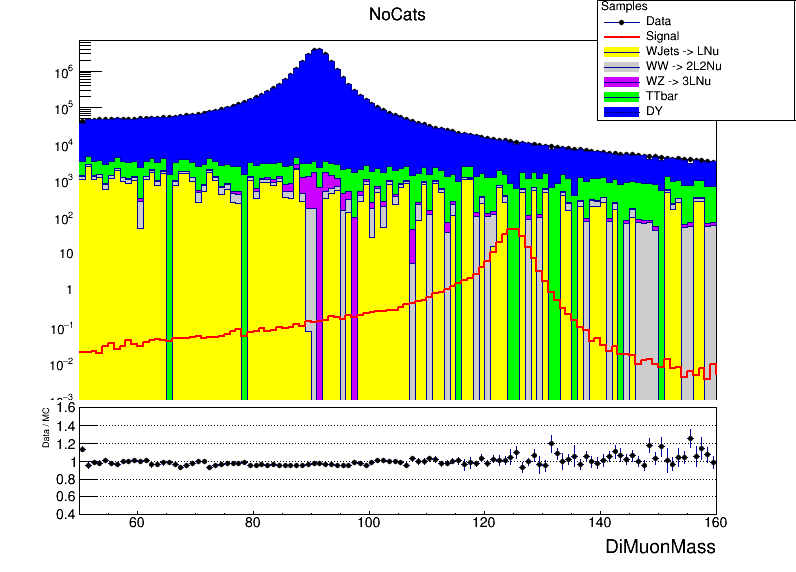
\includegraphics[width=0.8\textwidth, height=0.8\textheight]{figs/higgs/distributions/baseline_rochester/distribution__NoCats__DiMuonMass__logY.png}
    \end{center}
    % \PlaceText{25mm}{46mm}{\alert{$\Longrightarrow$}}
    % \PlaceText{5mm}{46mm}{\begin{tiny}\alert{Background/Data Level}\end{tiny}}
    % \PlaceText{25mm}{55mm}{\alert{$\Longrightarrow$}}
    % \PlaceText{5mm}{55mm}{\begin{tiny}\alert{Signal Level}\end{tiny}}
  \end{frame}

  \begin{frame}{Top Category: Corrected vs Uncorrected}
    \begin{center}
      Corrected (Rochester) vs Uncorrected:\\
      \vspace{0.5cm}
      % \begin{block}{Remark}
      %   Note the orders of magnitude difference between background and \alert{signal}!
      % \end{block}
      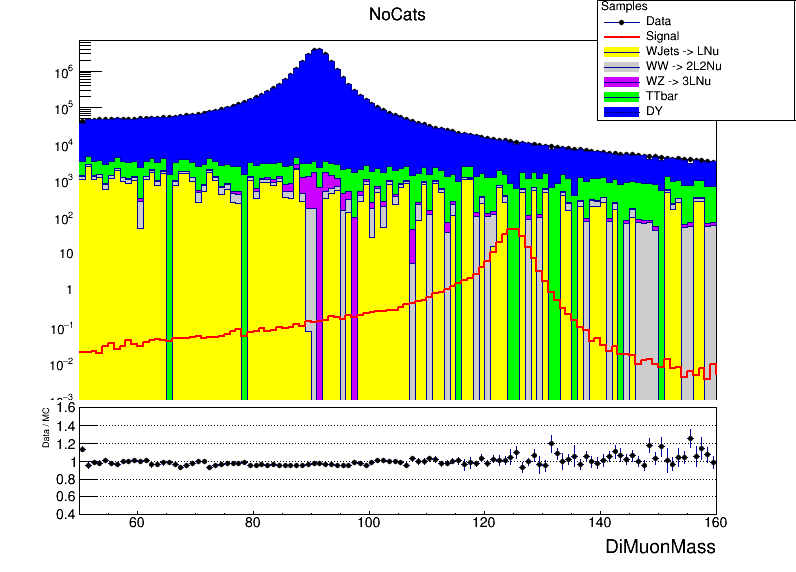
\includegraphics[width=0.5\textwidth, height=0.5\textheight]{figs/higgs/distributions/baseline_rochester/distribution__NoCats__DiMuonMass__logY.png}
      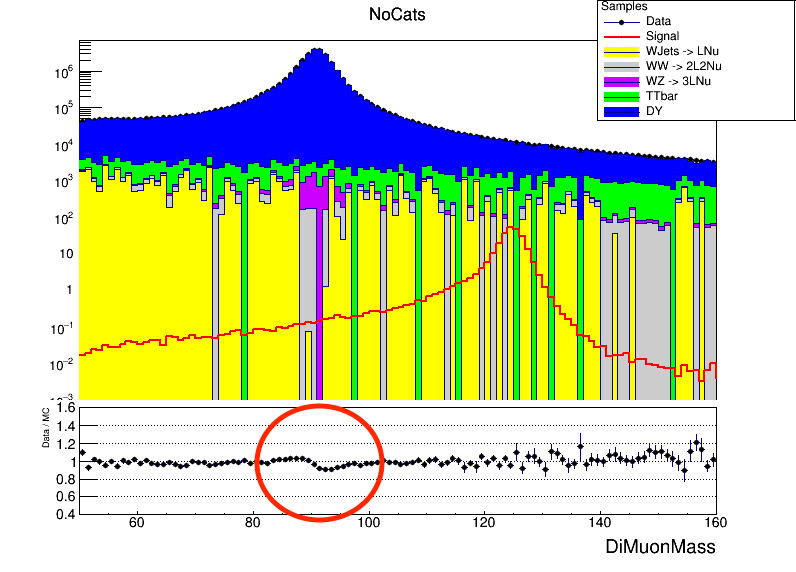
\includegraphics[width=0.5\textwidth, height=0.5\textheight]{figs/higgs/distributions/baseline_nocorrections/distribution__NoCats__DiMuonMass__logY.png}
    \end{center}
    % \PlaceText{25mm}{46mm}{\alert{$\Longrightarrow$}}
    % \PlaceText{5mm}{46mm}{\begin{tiny}\alert{Background/Data Level}\end{tiny}}
    % \PlaceText{25mm}{55mm}{\alert{$\Longrightarrow$}}
    % \PlaceText{5mm}{55mm}{\begin{tiny}\alert{Signal Level}\end{tiny}}
  \end{frame}

  \begin{frame}{Top Category: Kinematic Distributions}
    \begin{columns}[T]
      \begin{column}{0.5\textwidth}
        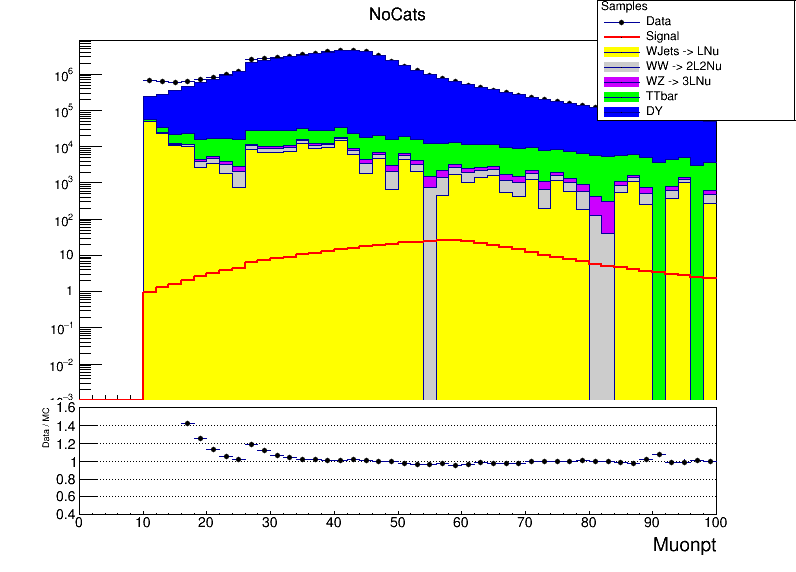
\includegraphics[width=0.99\textwidth, height=0.45\textheight]{figs/higgs/distributions/baseline_rochester/distribution__NoCats__Muonpt__logY.png}\\
        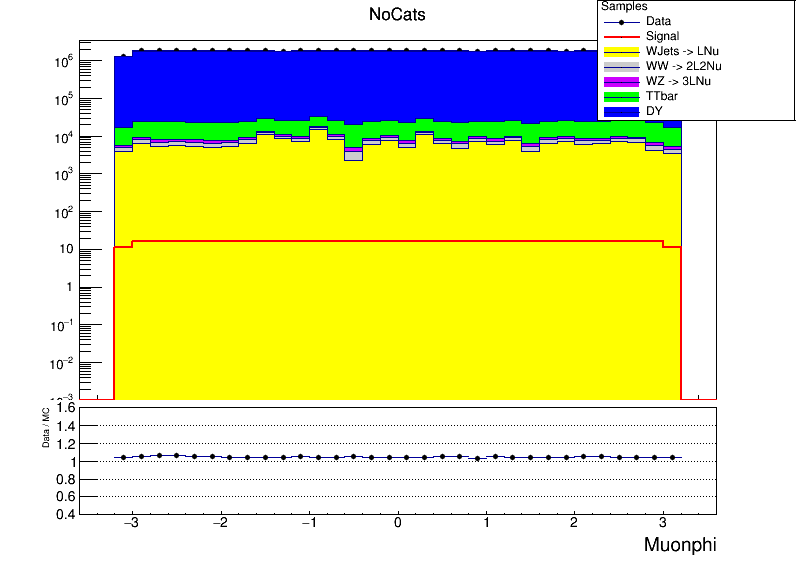
\includegraphics[width=0.99\textwidth, height=0.45\textheight]{figs/higgs/distributions/baseline_rochester/distribution__NoCats__Muonphi__logY.png}
      \end{column}
      \begin{column}{0.5\textwidth}
        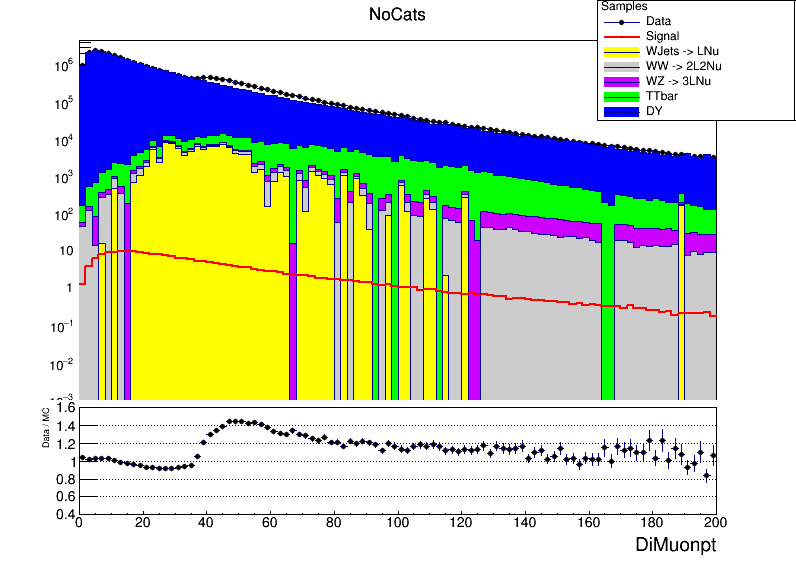
\includegraphics[width=0.99\textwidth, height=0.45\textheight]{figs/higgs/distributions/baseline_rochester/distribution__NoCats__DiMuonpt__logY.png}\\
        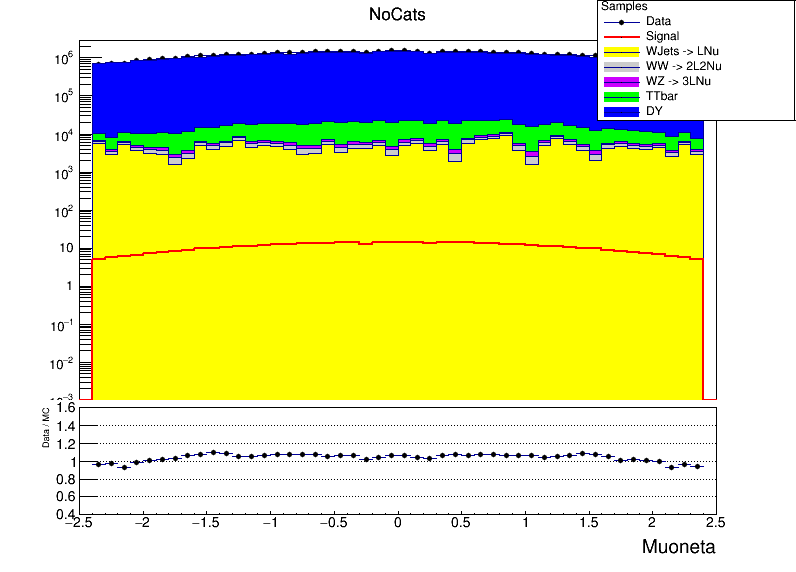
\includegraphics[width=0.99\textwidth, height=0.45\textheight]{figs/higgs/distributions/baseline_rochester/distribution__NoCats__Muoneta__logY.png}
      \end{column}
    \end{columns}
  \end{frame}

  \begin{frame}{Event Categorization}
    \begin{itemize}
      \item Grouping events using certain crteria
      \item 2 different procedures
      \item \alert{Baseline Categorization} is based on Run I categorization selections
      \item \alert{Greedy Categorization}: 2-step procedure
        \begin{itemize}
          \item Binary Classification: Engineer a new feature, BDT score, using Boostead Decision Tree (BDT)
          \item Greedy Event Grouping: Use 2 features (max($\eta_{\mu_1}$, $\eta_{\mu_2}$) and BDT score) to split events into different categories.
        \end{itemize}
    \end{itemize}
  \end{frame}

  \begin{frame}{Event Categorization: Baseline}
    \begin{itemize}
      \item Require only $m_{\mu\mu}$ in $[110, 160]$
      \item \alert{2Jet} Category
        \begin{itemize}
          \item \# Jets $>=2$
          \item $p_{t}^{j_1}>40$ GeV \&\& $p_{t}^{j_2}>30$ GeV \&\& $p_{t}^{MET}<40$ GeV
            \begin{itemize}
              \item if not satisfied, go to \alert{01Jet} Category part
              \item passed, then if $m_{jj}>650$ GeV \&\& $|d\eta|>3.5 \rightarrow$ \alert{VBFTIght} Category
              \item else if $m_{dijet}>250$ GeV \&\& $p_{t}^{\mu\mu}>50$ GeV $\rightarrow$ \alert{ggFTight} Category
              \item else $\rightarrow$ \alert{ggFLoose} Category
            \end{itemize}
        \end{itemize}
      \item \alert{01Jet} Category
        \begin{itemize}
          \item \# Jets $<=1$
          \item if $p_{t}^{\mu\mu} \ge 25$ GeV $\rightarrow$ \alert{01JetsTight} $\rightarrow$ Geometry Categorization
          \item else $\rightarrow$ \alert{01JetsLoose} $\rightarrow$ Geometry Categorization
        \end{itemize}
    \end{itemize}
  \end{frame}

  \begin{frame}{Event Categorization: Greedy Step1 - Binary Classification}
    \begin{itemize}
      \item Require only $m_{\mu\mu}$ in $[110, 160]$ GeV mass range
      \item Train a Boosted Decision Tree to perform a binary classification: signal / background.
      \item Training / Cross-Validation / Testing using half of Signal and all of Background events
      \item BDT Features are various event and kinematic variables: $p_{t}^{\mu\mu}$, $\eta_{\mu\mu}$, \# jets, \dots
        \begin{itemize}
          \item \alert{No mass dependence among the BDT features!}
        \end{itemize}
      \item BDT score (continuous value [-1, 1]) is preserved - do not actually select the ''turning point'' (for binary classification).
    \end{itemize}
  \end{frame}

  \begin{frame}{Event Categorization: Greedy Step1 - BDT ROC}
    \begin{center}
      BDT Receiver Operating Curve:
      % \begin{block}{Remark}
      %   Note the orders of magnitude difference between background and \alert{signal}!
      % \end{block}
      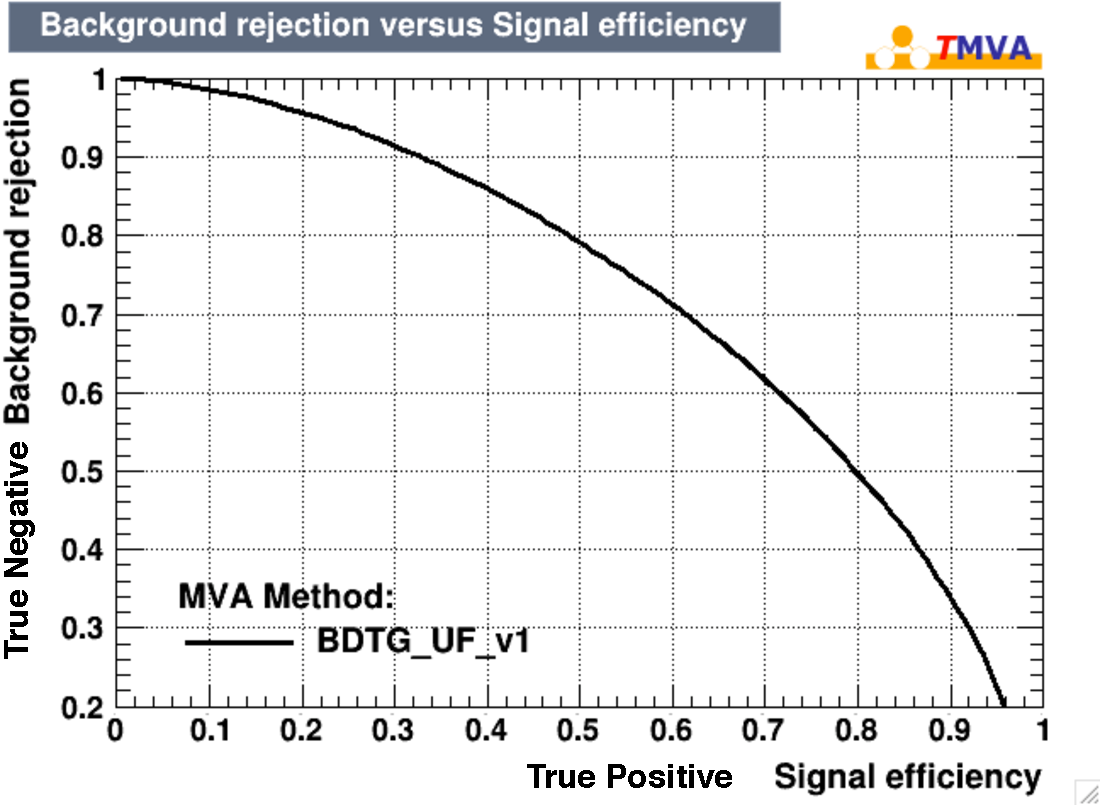
\includegraphics[width=0.8\textwidth, height=0.8\textheight]{figs/higgs/bdt_training/BDT_ROC_ge0j_all.pdf}
    \end{center}
    % \PlaceText{25mm}{46mm}{\alert{$\Longrightarrow$}}
    % \PlaceText{5mm}{46mm}{\begin{tiny}\alert{Background/Data Level}\end{tiny}}
    % \PlaceText{25mm}{55mm}{\alert{$\Longrightarrow$}}
    % \PlaceText{5mm}{55mm}{\begin{tiny}\alert{Signal Level}\end{tiny}}
  \end{frame}

  \begin{frame}{Event Categorization: Greedy Step2 - Event Splitting}
    \begin{columns}[T]
      \begin{column}{0.6\textwidth}
        Define a Significance, $S_c$, for a histogram:\\
        \begin{equation}
          {S^2_c} = \sum_{c,i}N^{S2}_{c,i}/N^{B}_{c,i}
          \label{eq:higgs_categorization_significance}
        \end{equation}
        Use 2 features: max($\eta_{\mu_1}$, $\eta_{\mu_2}$) and BDT score
        Define a Gain, G, of a split:
        \begin{equation}
          {G} = {S^2_{left}} + {S^2_{right}} - {S^2_{node}}
          \label{eq:higgs_categorization_gain}
        \end{equation}
        \begin{itemize}
          \item For a given histogram, greedily scan through the features\\
          \item Pick the split that maximizes Gain\\
          \item Proceed recursively.
        \end{itemize}
      \end{column}
      \begin{column}{0.4\textwidth}
        \alert{Top Category} Mass Distribution:\\\vspace{0.2cm}
        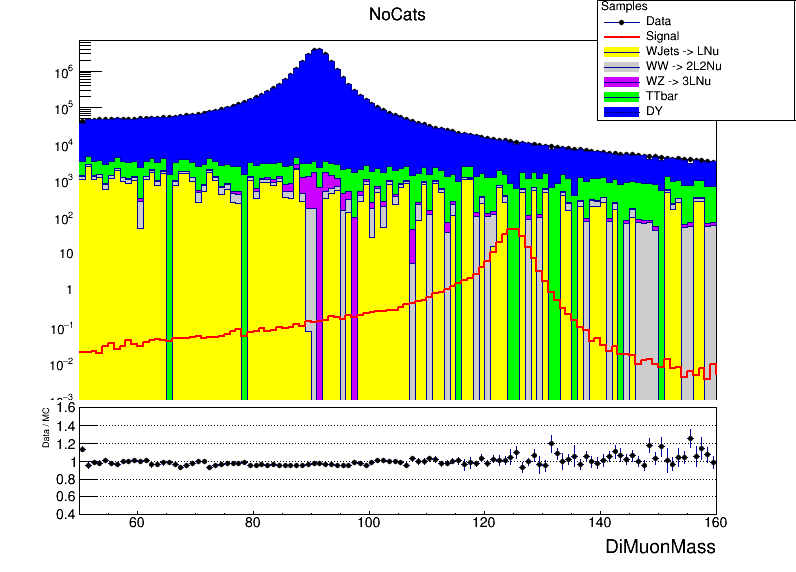
\includegraphics[width=0.99\textwidth, height=0.45\textheight]{figs/higgs/distributions/baseline_rochester/distribution__NoCats__DiMuonMass__logY.png}
      \end{column}
    \end{columns}
    \vspace{0.2cm}
    \alert{The result is 13 categories (15 for Baseline) that are obtained via a greedy procedure!}
  \end{frame}

  \begin{frame}{Event Categorization: Greedy - Mass Distributions}
    \begin{center}
      Most Sensitive Category ''c12'':\\\vspace{0.2cm}
      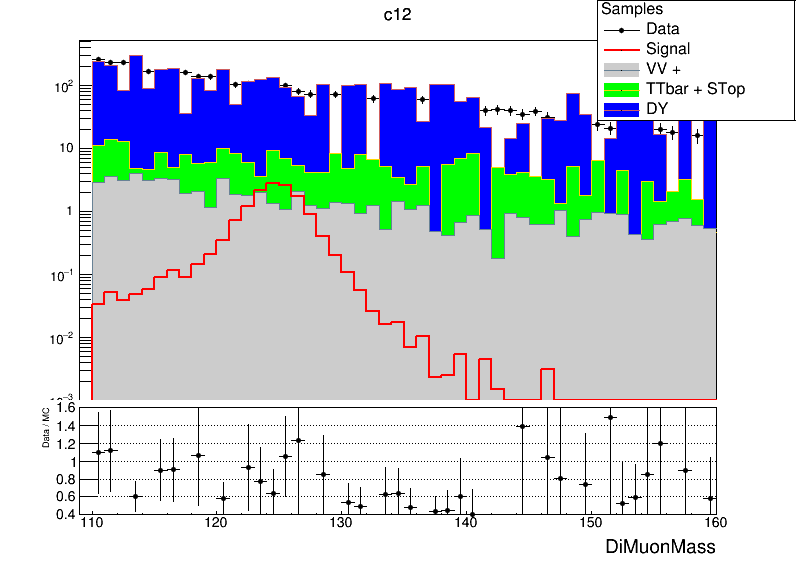
\includegraphics[width=0.8\textwidth, height=0.8\textheight]{figs/higgs/distributions/bdt_uf/distribution__c12__DiMuonMass__logY.png}
    \end{center}
  \end{frame}

  \begin{frame}{Event Categorization: Greedy - Mass Distributions}
    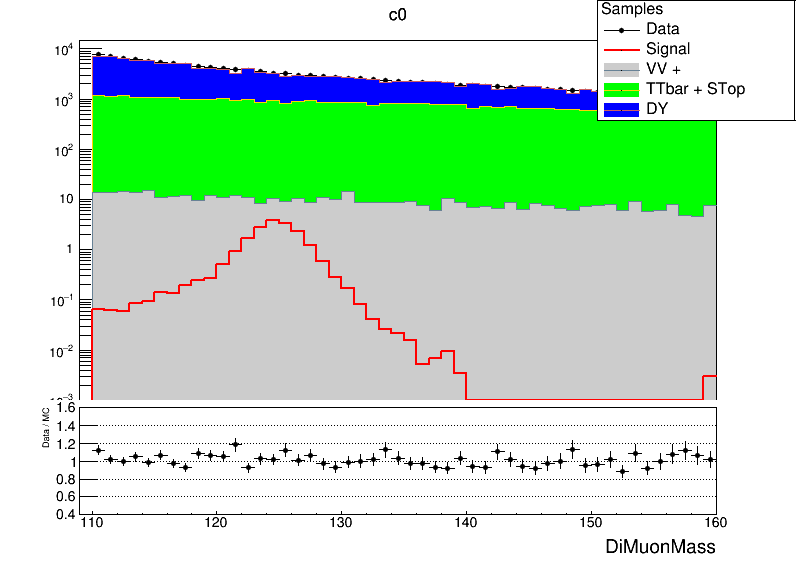
\includegraphics[width=0.49\textwidth, height=0.45\textheight]{figs/higgs/distributions/bdt_uf/distribution__c0__DiMuonMass__logY.png}
    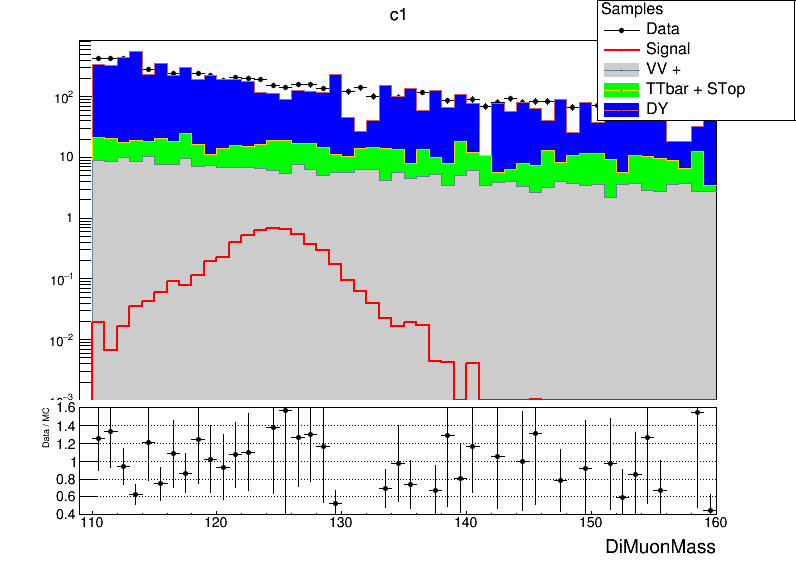
\includegraphics[width=0.49\textwidth, height=0.45\textheight]{figs/higgs/distributions/bdt_uf/distribution__c1__DiMuonMass__logY.png}\\
    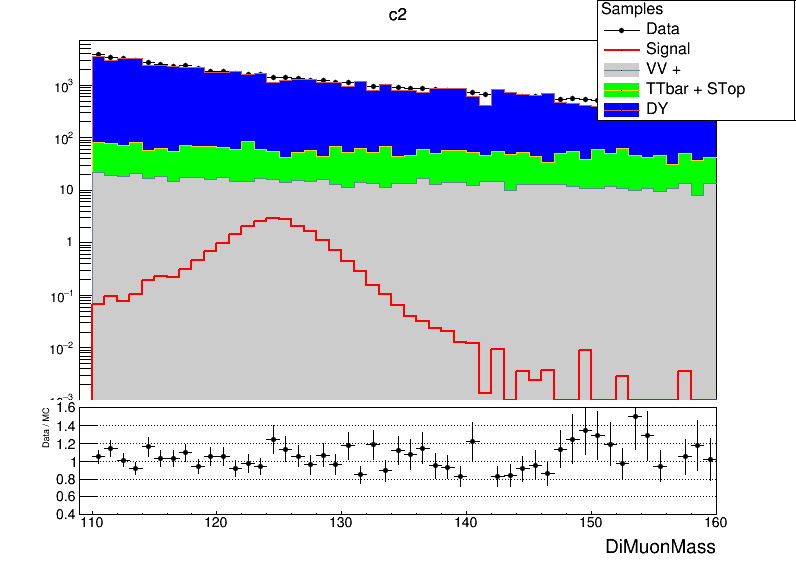
\includegraphics[width=0.49\textwidth, height=0.45\textheight]{figs/higgs/distributions/bdt_uf/distribution__c2__DiMuonMass__logY.png}
    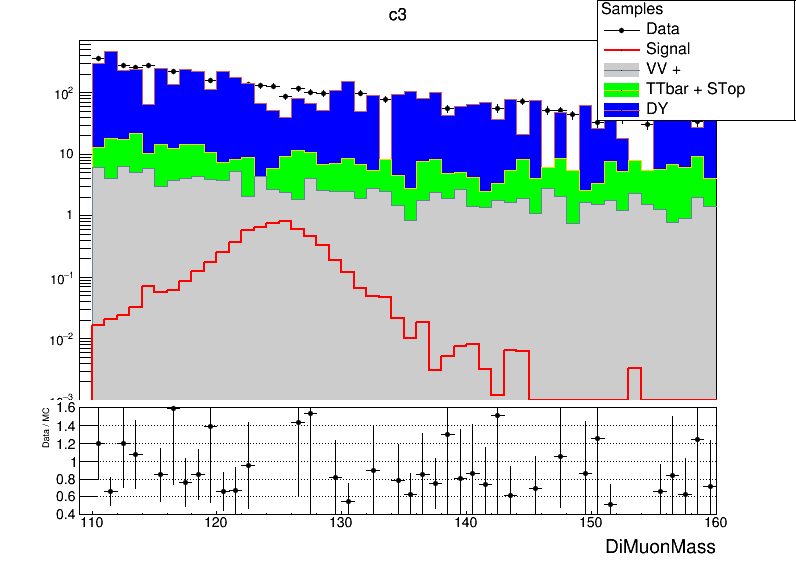
\includegraphics[width=0.49\textwidth, height=0.45\textheight]{figs/higgs/distributions/bdt_uf/distribution__c3__DiMuonMass__logY.png}
  \end{frame}

  \begin{frame}{Event Categorization: Greedy - Mass Distributions}
    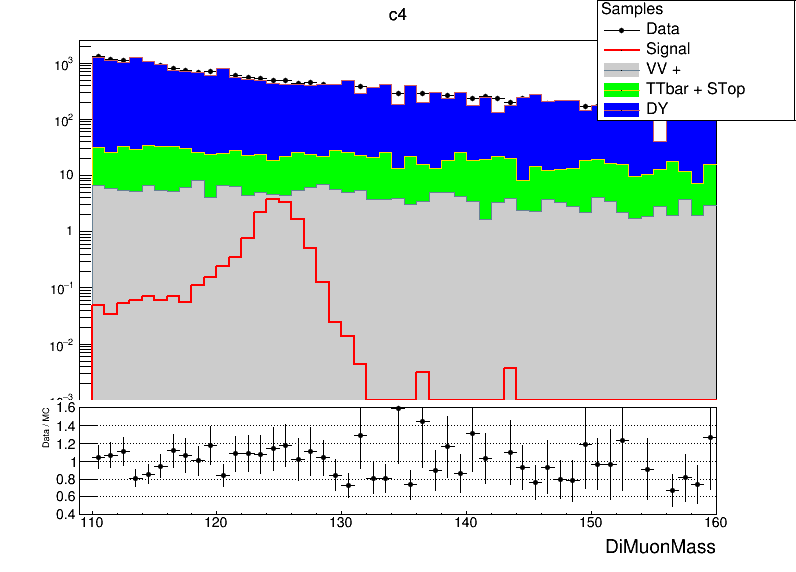
\includegraphics[width=0.49\textwidth, height=0.45\textheight]{figs/higgs/distributions/bdt_uf/distribution__c4__DiMuonMass__logY.png}
    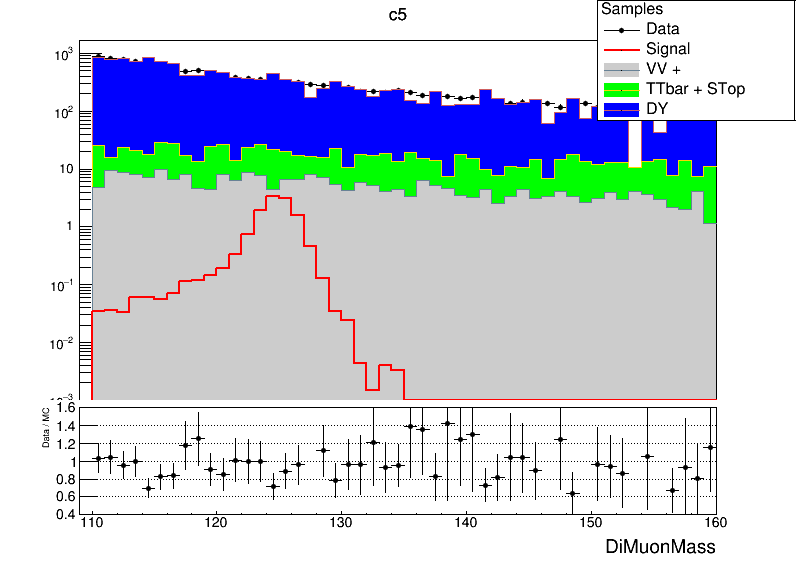
\includegraphics[width=0.49\textwidth, height=0.45\textheight]{figs/higgs/distributions/bdt_uf/distribution__c5__DiMuonMass__logY.png}\\
    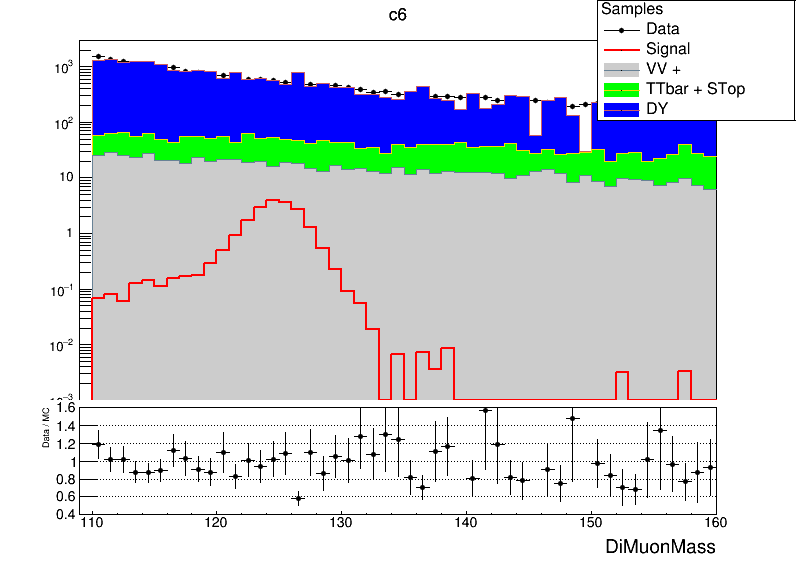
\includegraphics[width=0.49\textwidth, height=0.45\textheight]{figs/higgs/distributions/bdt_uf/distribution__c6__DiMuonMass__logY.png}
    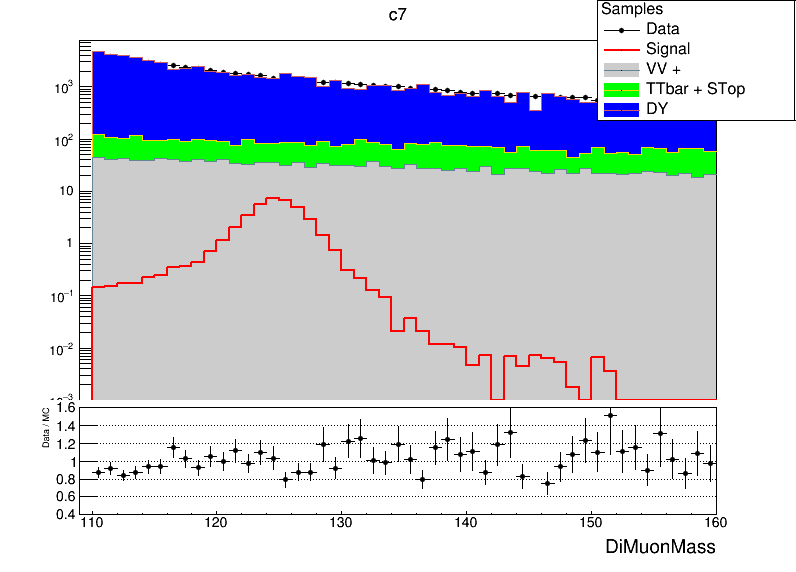
\includegraphics[width=0.49\textwidth, height=0.45\textheight]{figs/higgs/distributions/bdt_uf/distribution__c7__DiMuonMass__logY.png}
  \end{frame}

  \begin{frame}{Event Categorization: Greedy - Mass Distributions}
    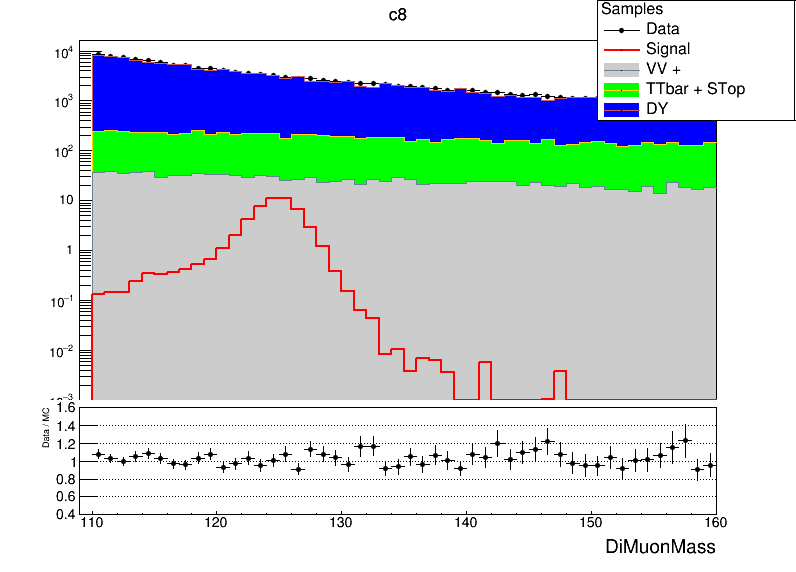
\includegraphics[width=0.49\textwidth, height=0.45\textheight]{figs/higgs/distributions/bdt_uf/distribution__c8__DiMuonMass__logY.png}
    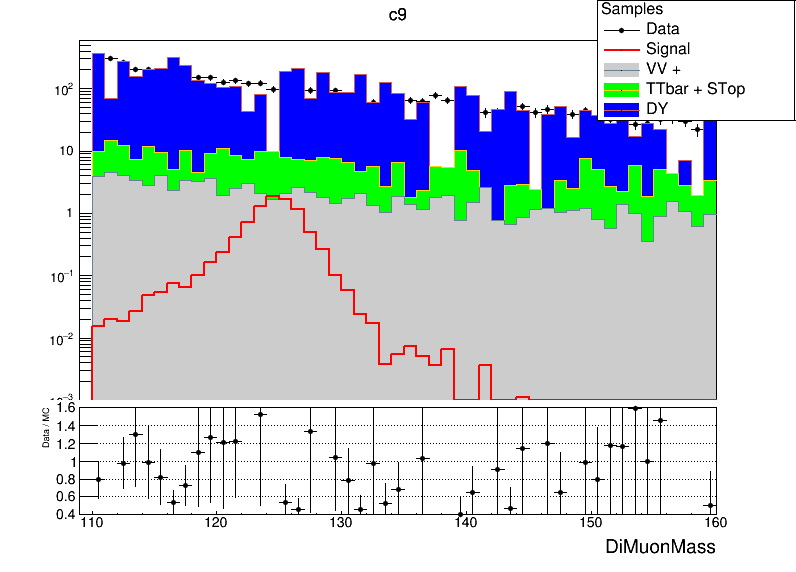
\includegraphics[width=0.49\textwidth, height=0.45\textheight]{figs/higgs/distributions/bdt_uf/distribution__c9__DiMuonMass__logY.png}\\
    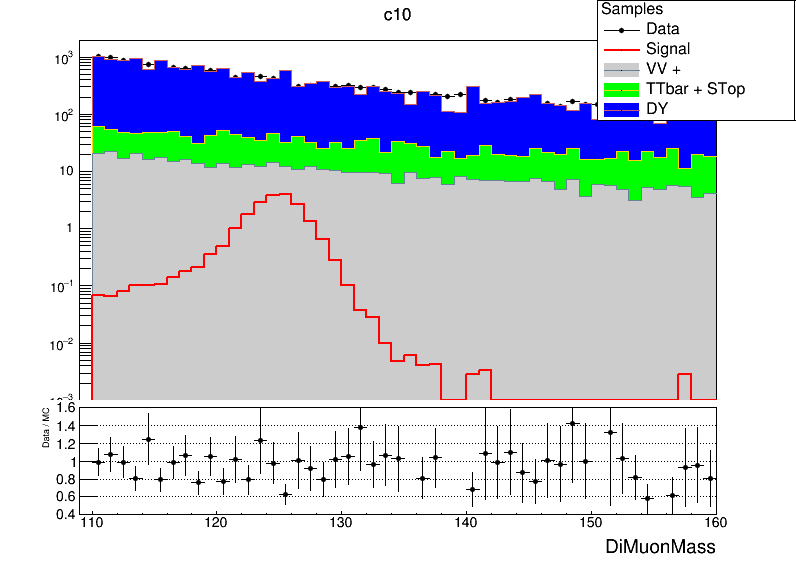
\includegraphics[width=0.49\textwidth, height=0.45\textheight]{figs/higgs/distributions/bdt_uf/distribution__c10__DiMuonMass__logY.png}
    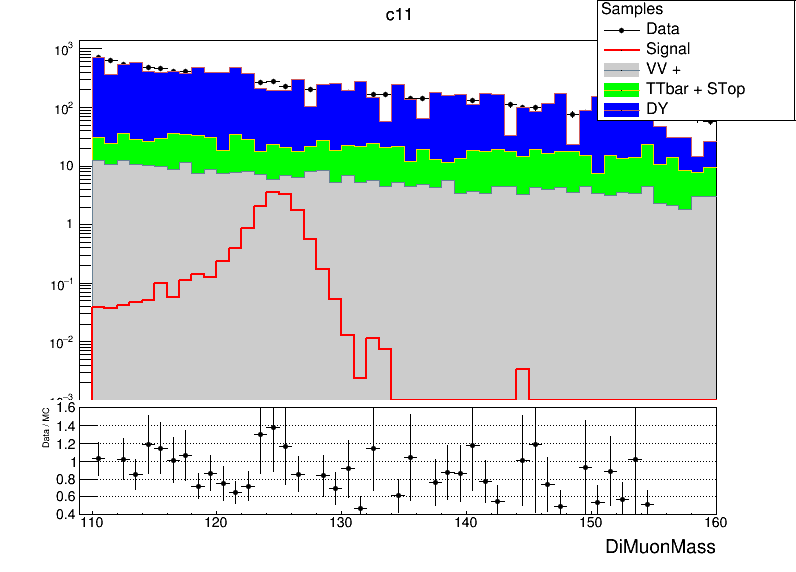
\includegraphics[width=0.49\textwidth, height=0.45\textheight]{figs/higgs/distributions/bdt_uf/distribution__c11__DiMuonMass__logY.png}
  \end{frame}

  % \begin{frame}{Signal Modeling}
  % \end{frame}

  \begin{frame}{Signal Model: Basics}
        \textbf{-} Triple Gaussian PDF:\\\vspace{-0.4cm}
        \begin{align}
          S(x, m_{H}, \theta) &= f_{1} \mathcal{N}_{1}(x, \mu_{1}, \sigma_{1}) + (1-f_{1}) \left(f_{2} \mathcal{N}_{2}(x, \mu_{2}, \sigma_{2}) + (1-f_{2}) \mathcal{N}_{3}(x, \mu_{3}, \sigma_{3})\right)
        \end{align}
        \textbf{-} Each production process treated separately\\\vspace{0.2cm}
        \textbf{-} MC mass distributions are fitted and all model parameters are fixed\\\vspace{0.2cm}
        \textbf{-} Total Signal Normalization, the SM yield, is fixed:\\\vspace{-0.4cm}
        \begin{align}
          \text{Yield} = \mathcal{L}\,\sigma(pp\rightarrow H)\, \mathcal{B}(H \rightarrow \mu\mu) \, \varepsilon A
        \end{align}
        \begin{center}
        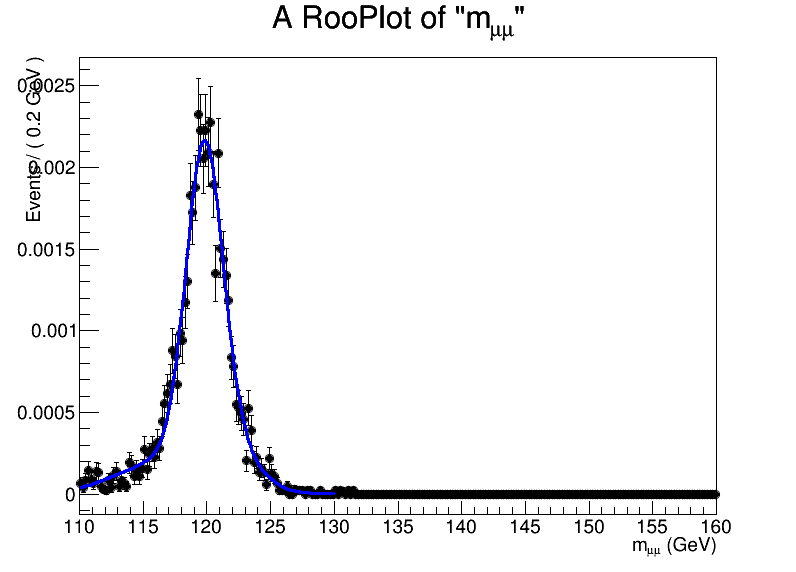
\includegraphics[width=0.3\textwidth, height=0.3\textheight]{figs/higgs/signalmodel/bdt/bdt_110to160_withSys/signalFit__c0__120__GluGlu__TripleGaus__default.png}
        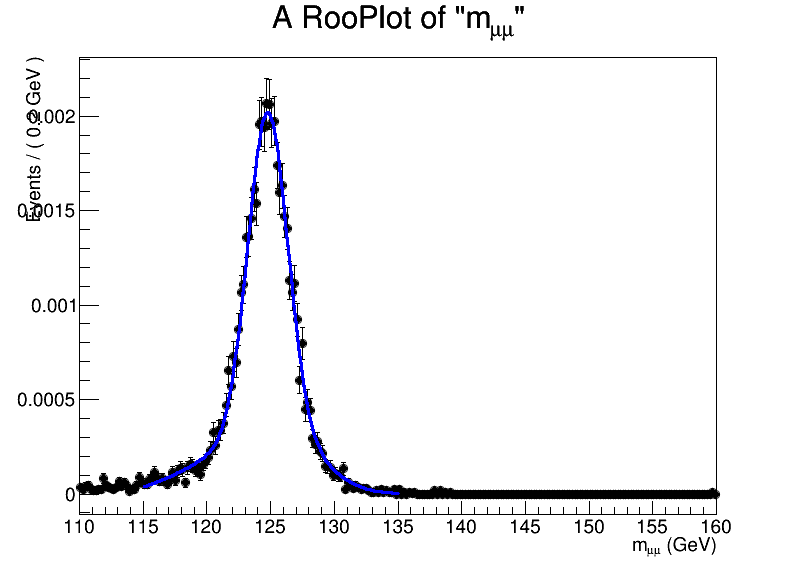
\includegraphics[width=0.3\textwidth, height=0.3\textheight]{figs/higgs/signalmodel/bdt/bdt_110to160_withSys/signalFit__c0__125__GluGlu__TripleGaus__default.png}
        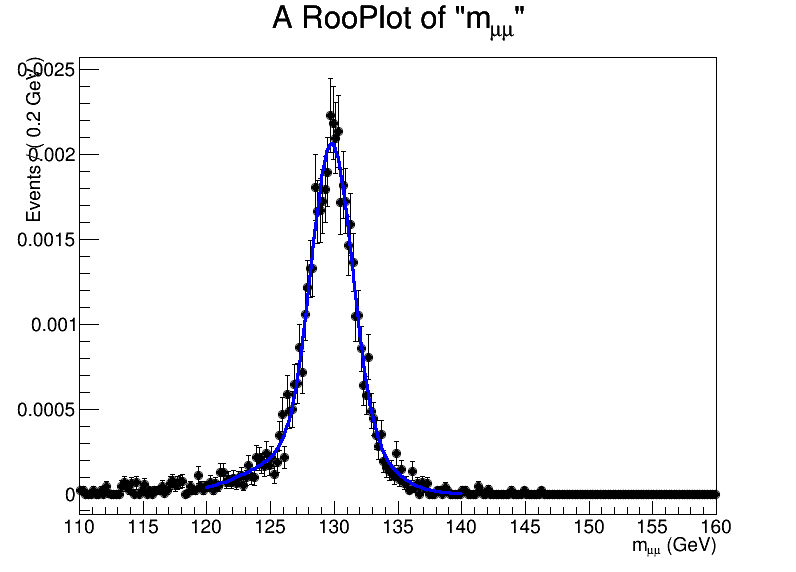
\includegraphics[width=0.3\textwidth, height=0.3\textheight]{figs/higgs/signalmodel/bdt/bdt_110to160_withSys/signalFit__c0__130__GluGlu__TripleGaus__default.png}
        \end{center}
  \end{frame}

  \begin{frame}{Signal Model: Examples}
    \vspace{-0.7cm}
    \begin{columns}[T]
      \begin{column}{0.33\textwidth}
        \begin{center}
          \tiny{Category ''c0'' Gluon Fusion}\\
          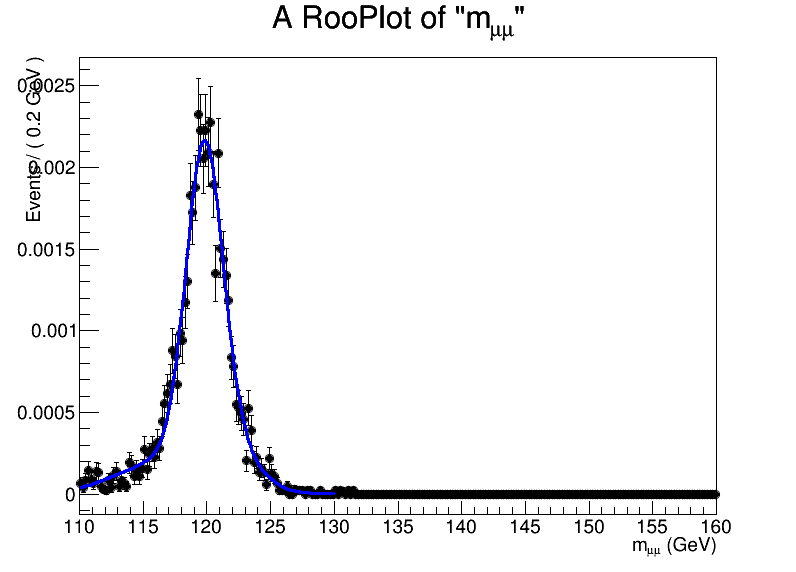
\includegraphics[width=0.95\textwidth, height=0.3\textheight]{figs/higgs/signalmodel/bdt/bdt_110to160_withSys/signalFit__c0__120__GluGlu__TripleGaus__default.png}\\
          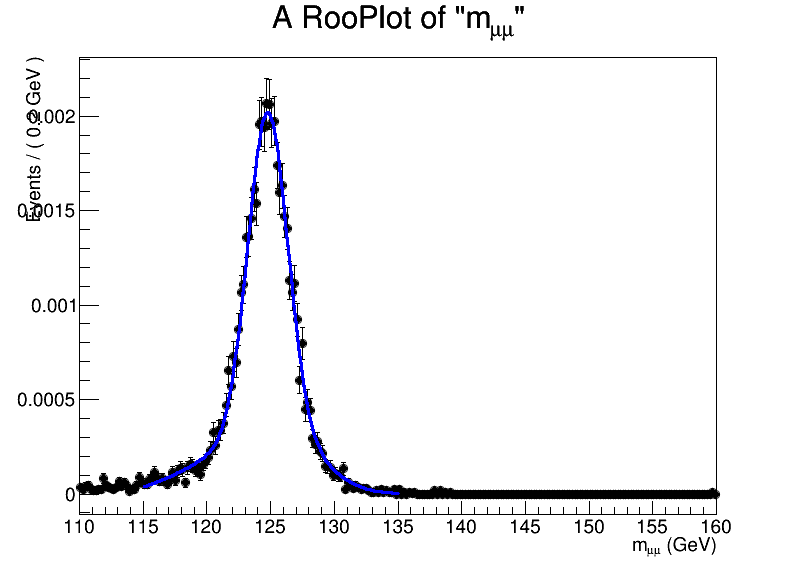
\includegraphics[width=0.95\textwidth, height=0.3\textheight]{figs/higgs/signalmodel/bdt/bdt_110to160_withSys/signalFit__c0__125__GluGlu__TripleGaus__default.png}\\
          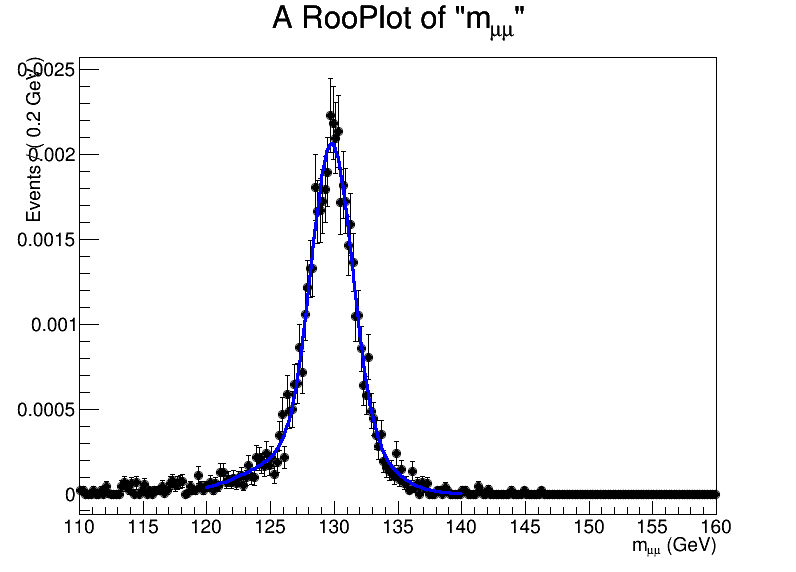
\includegraphics[width=0.95\textwidth, height=0.3\textheight]{figs/higgs/signalmodel/bdt/bdt_110to160_withSys/signalFit__c0__130__GluGlu__TripleGaus__default.png}
        \end{center}
      \end{column}
      \begin{column}{0.33\textwidth}
        \begin{center}
          \tiny{Category ''c0'' Vector Boson Fusion}\\
          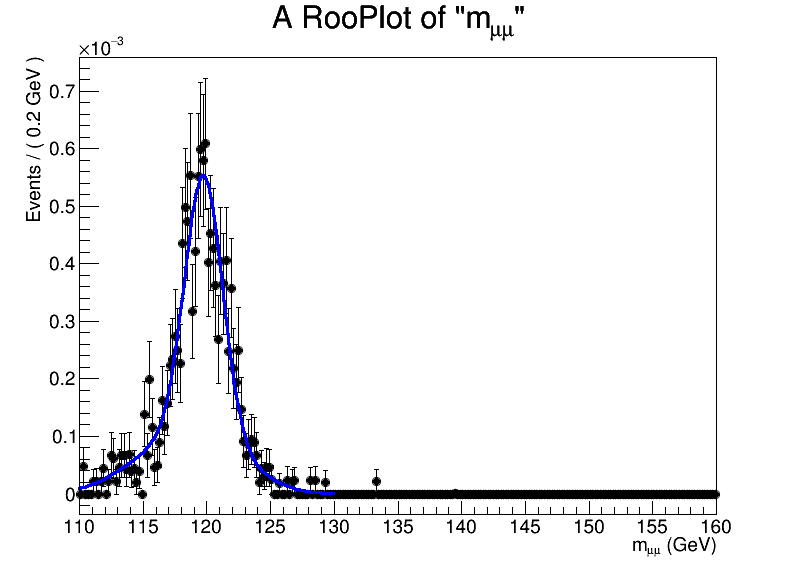
\includegraphics[width=0.95\textwidth, height=0.3\textheight]{figs/higgs/signalmodel/bdt/bdt_110to160_withSys/signalFit__c0__120__VBF__TripleGaus__default.png}\\
          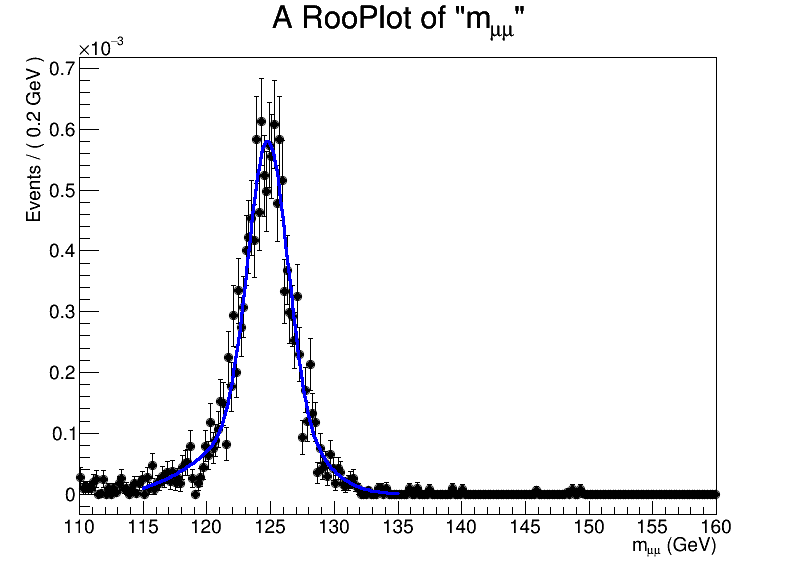
\includegraphics[width=0.95\textwidth, height=0.3\textheight]{figs/higgs/signalmodel/bdt/bdt_110to160_withSys/signalFit__c0__125__VBF__TripleGaus__default.png}\\
          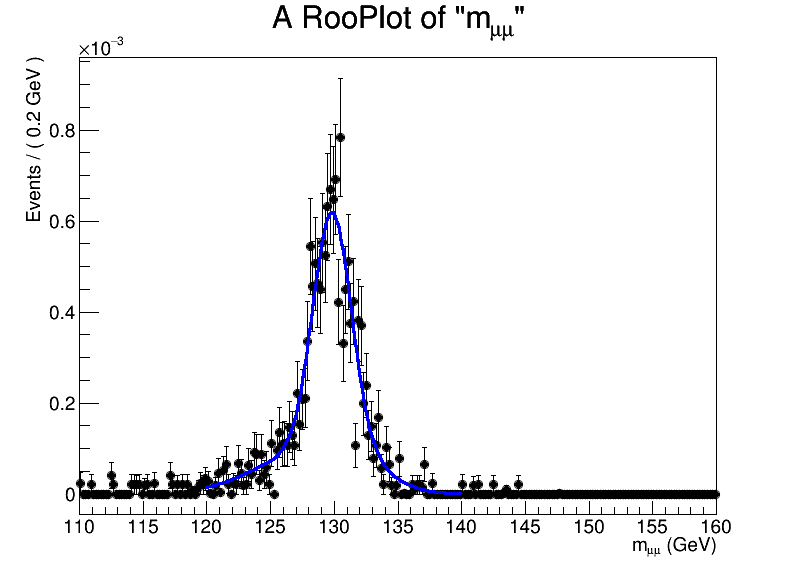
\includegraphics[width=0.95\textwidth, height=0.3\textheight]{figs/higgs/signalmodel/bdt/bdt_110to160_withSys/signalFit__c0__130__VBF__TripleGaus__default.png}
        \end{center}
      \end{column}
      \begin{column}{0.33\textwidth}
        \begin{center}
          \tiny{Category ''c1'' Gluon Fusion Fusion}\\
          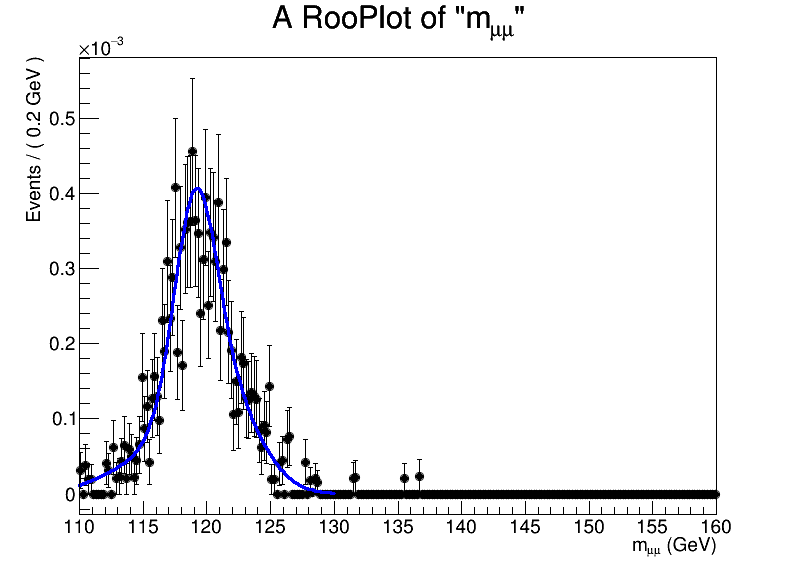
\includegraphics[width=0.95\textwidth, height=0.3\textheight]{figs/higgs/signalmodel/bdt/bdt_110to160_withSys/signalFit__c1__120__GluGlu__TripleGaus__default.png}\\
          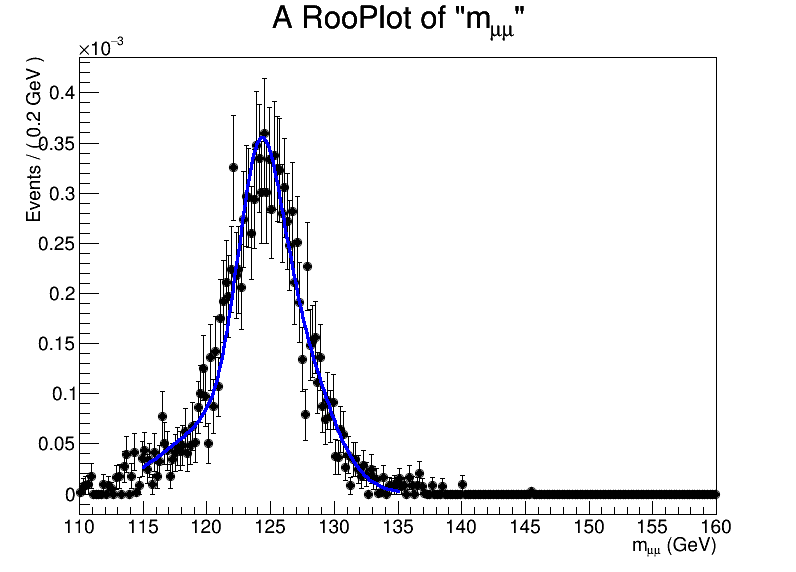
\includegraphics[width=0.95\textwidth, height=0.3\textheight]{figs/higgs/signalmodel/bdt/bdt_110to160_withSys/signalFit__c1__125__GluGlu__TripleGaus__default.png}\\
          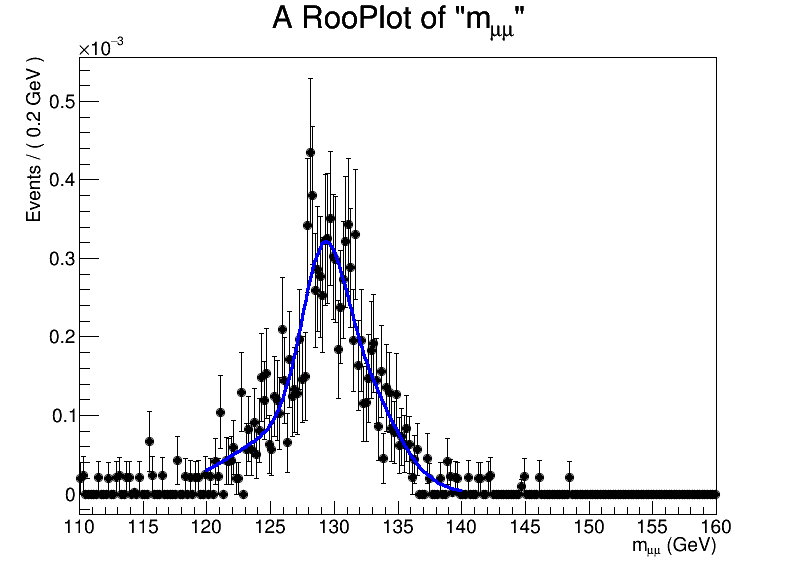
\includegraphics[width=0.95\textwidth, height=0.3\textheight]{figs/higgs/signalmodel/bdt/bdt_110to160_withSys/signalFit__c1__130__GluGlu__TripleGaus__default.png}
        \end{center}
      \end{column}
    \end{columns}
  \end{frame}

    \begin{frame}[c]{Signal Model: Mass Interpolation}
    \vspace{-0.7cm}
    \begin{columns}[T]
      \begin{column}{0.4\textwidth}
        \begin{center}
          \tiny{Category ''c0'' Gluon Fusion}\\
          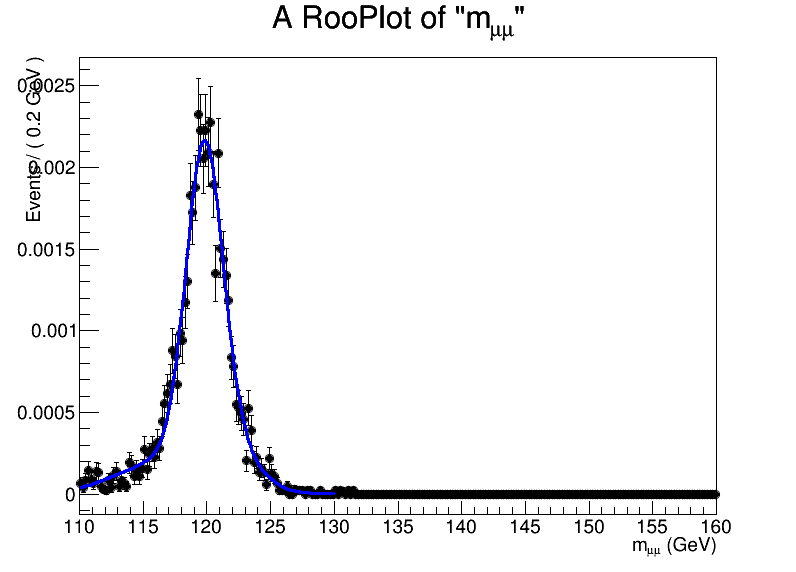
\includegraphics[width=0.95\textwidth, height=0.3\textheight]{figs/higgs/signalmodel/bdt/bdt_110to160_withSys/signalFit__c0__120__GluGlu__TripleGaus__default.png}\\
          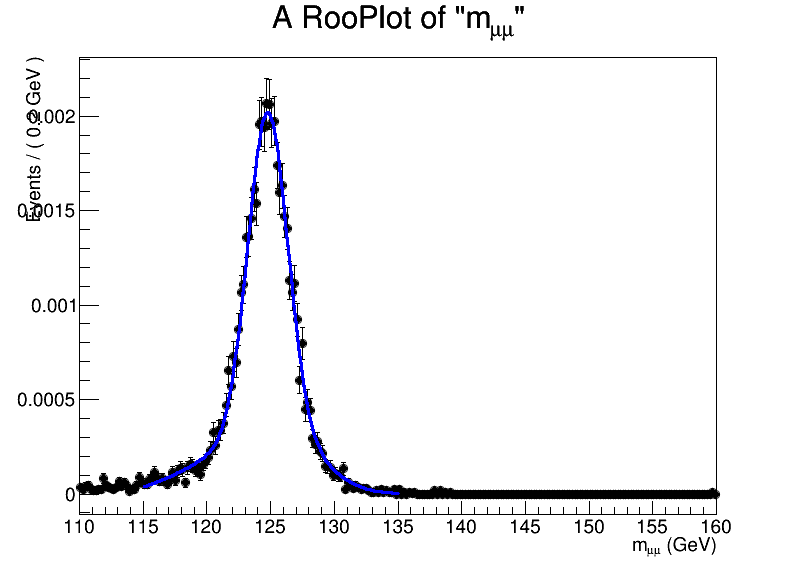
\includegraphics[width=0.95\textwidth, height=0.3\textheight]{figs/higgs/signalmodel/bdt/bdt_110to160_withSys/signalFit__c0__125__GluGlu__TripleGaus__default.png}\\
          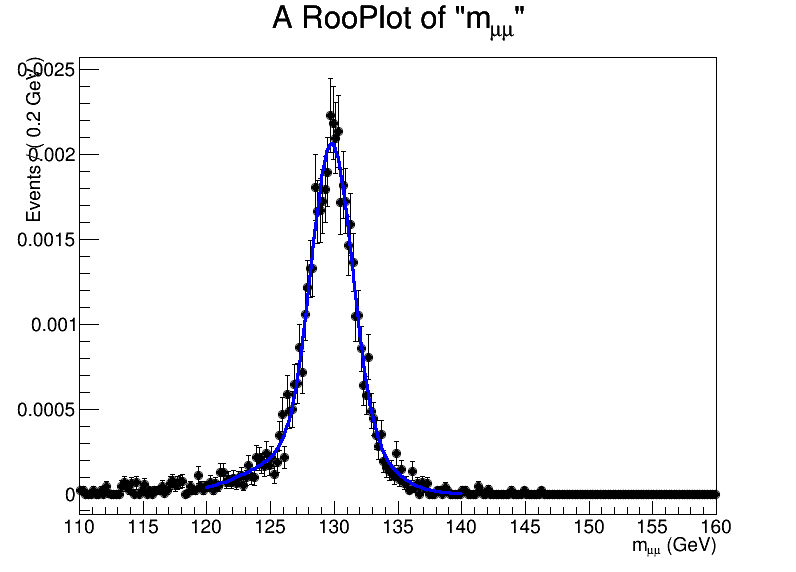
\includegraphics[width=0.95\textwidth, height=0.3\textheight]{figs/higgs/signalmodel/bdt/bdt_110to160_withSys/signalFit__c0__130__GluGlu__TripleGaus__default.png}
        \end{center}
      \end{column}
      \begin{column}{0.6\textwidth}
        \begin{center}
          \begin{itemize}
            \item \tiny{The search is performed in the mass range [120, 130] GeV.}
            \item \tiny{3 mass points used for parameter interpolation: 120, 125, 130 GeV}
            \item \tiny{Parameters of individual models are fitted and then interpolated in between as function of the Higgs mass.}
          \end{itemize}
          \vspace{0.5cm}
          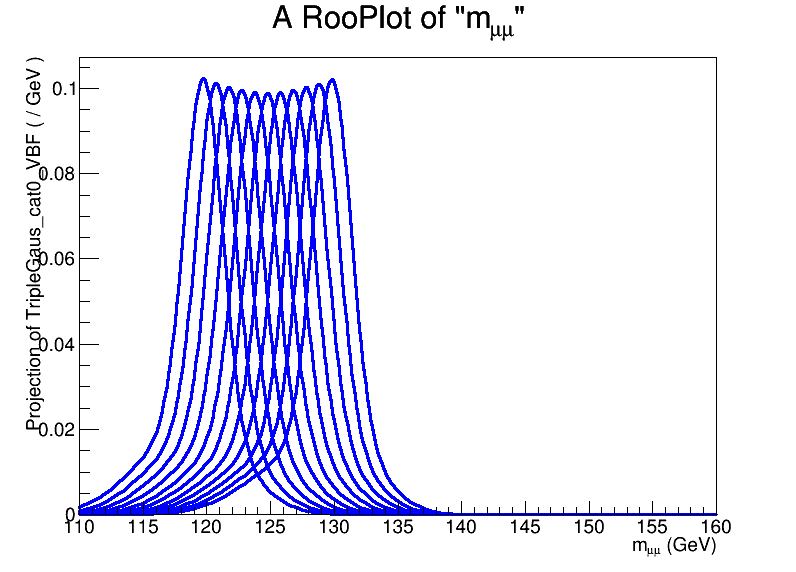
\includegraphics[width=0.95\textwidth, height=0.65\textheight]{figs/higgs/signalmodel/bdt/bdt_110to160_withSys/signalFitInterpolationWithSpline__c0__VBF__TripleGaus__.png}
        \end{center}
      \end{column}
    \end{columns}
  \end{frame}

  \begin{frame}{Background Model}
    \begin{itemize}
      \item Data-driven approach - providing actual mathematical functions as pdf candidates
      \item 2 types of models: \textbf{Physics-motivated}  and \textbf{Order-dependent}
      \item \textbf{Order-dependent} - various polynomial-like series
      \item Background is left completely floating - all parameters of the model are floating!
      \item Employ an envelope method - build a set of functions and use them simultaneously for the fitting procedure.
      \item Envelope method $\rightarrow$ simplify the bias estimation
    \end{itemize}
  \end{frame}

  \begin{frame}{Background Model}
    \textbf{-} Physics-motivated functional forms:\\\vspace{-0.2cm}
    \begin{align}
        \textit{ExpPolynomial: } {B(x)}& = {e^{a_{1}x + a_{2}x^2}} \\
        \textit{BWZ: } {B(x)}& = {\frac{e^{ax}\sigma_{z}}{(x-\mu_{z})^2 + (\frac{\sigma_{z}}{2})^2}} \\
        \textit{BWZRedux: } {B(x)}& = {\frac{e^{a_{2}x + a_{3}x^2}}{(x-\mu_{z})^{a_{1}} + (\frac{2.5}{2})^{a_{1}}}} \\
        \textit{BWZGamma: } {B(x)}& = {f\frac{e^{ax}\sigma_{z}}{(x-\mu_{z})^2 + (\frac{\sigma_{z}}{2})^2} + (1-f)\frac{e^{ax}}{x^2}}
    \end{align}
  \end{frame}

  \begin{frame}{Background Model}
    \textbf{-} Various order-dependent functional forms:\\\vspace{0.02cm}
    \textbf{-} Order is selected by using F-Test (Fisher Test) procedure\\\vspace{-0.2cm}
    \begin{align}
        \textit{Bernsteins: } {B(x)}& = {\sum_{i=0}^{n} \alpha_i[\binom{n}{i}x^{i}(1-x)^{n-i}]} \\
        \textit{SumExponentials: } {B(x)}& = {\sum_{i=1}^{n} \beta_{i}e^{\alpha_{i}x}}\\
        \textit{SumPowers: } {B(x)}& = {\sum_{i=1}^{n} \beta_{i}x^{\alpha_{i}}}\\
        \textit{LaurentSeries: } {B(x)}& = {\sum_{i} \alpha_{i}x^{i}}
    \end{align}
  \end{frame}

  \begin{frame}[c]{Background Model: Examples}
    \vspace{-0.7cm}
    \begin{columns}[T]
      \begin{column}{0.5\textwidth}
        \begin{center}
        Example of an envelope of background functions for \textbf{c12}\\
        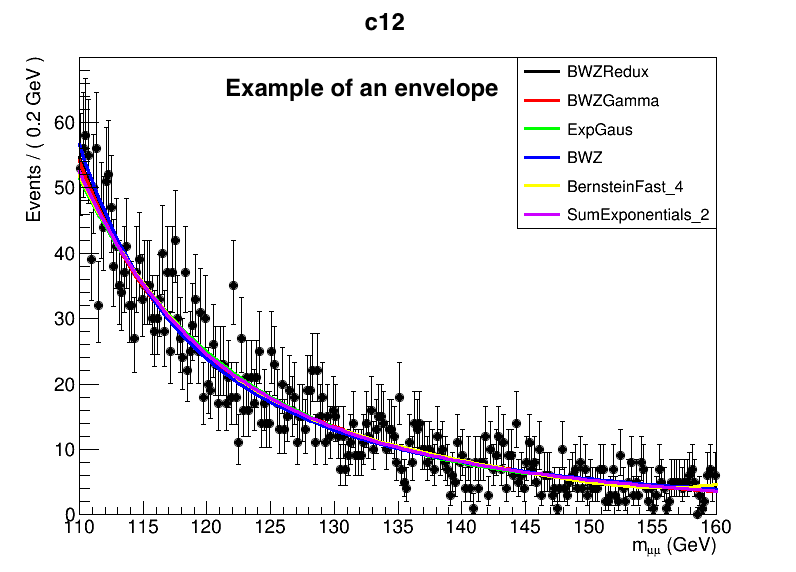
\includegraphics[width=0.95\textwidth, height=0.5\textheight]{figs/higgs/backgroundmodel/uf_bdt/backgroundFits__c12__bkgModels.png}
        \end{center}
      \end{column}
      \begin{column}{0.5\textwidth}
        \begin{center}
        Example of the Fisher Test for Bernstein Polynomials for \textbf{c12}\\
        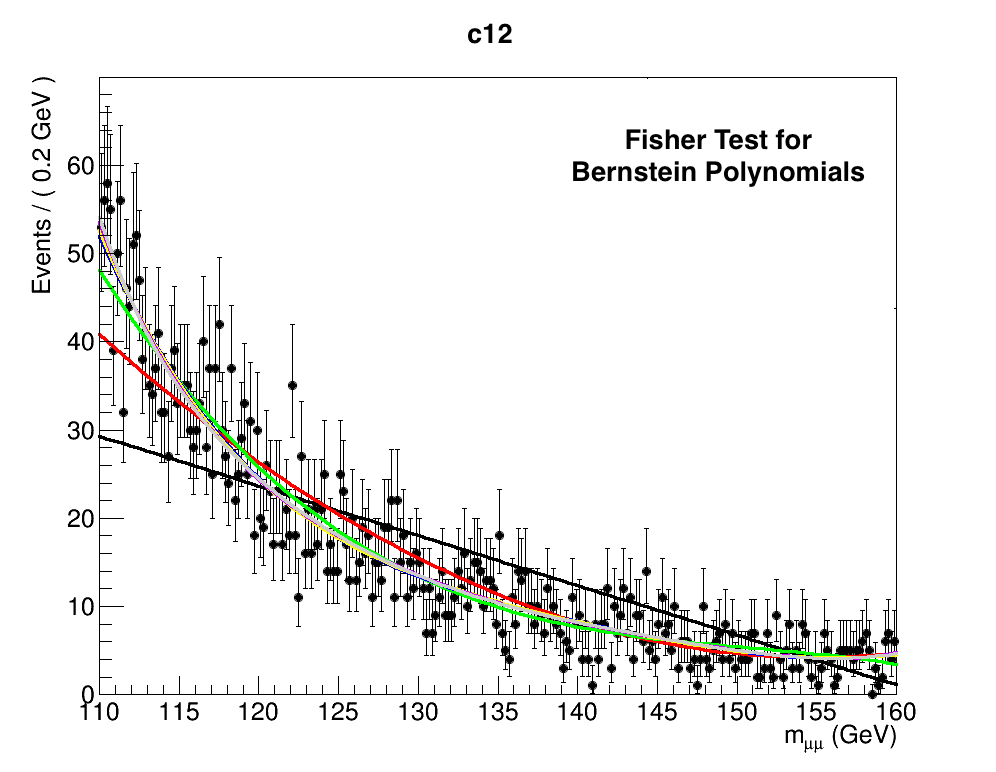
\includegraphics[width=0.95\textwidth, height=0.5\textheight]{figs/higgs/ftest/uf/ftest__c12__bernsteinFastModels.png}
        \end{center}
      \end{column}
    \end{columns}
  \end{frame}

  \begin{frame}{Background Model: c0 - c3}
    \includegraphics[width=0.49\textwidth, height=0.45\textheight]{figs/higgs/backgroundmodel/uf_bdt/backgroundFits__c0__bkgModels.png}
    \includegraphics[width=0.49\textwidth, height=0.45\textheight]{figs/higgs/backgroundmodel/uf_bdt/backgroundFits__c1__bkgModels.png}\\
    \includegraphics[width=0.49\textwidth, height=0.45\textheight]{figs/higgs/backgroundmodel/uf_bdt/backgroundFits__c2__bkgModels.png}
    \includegraphics[width=0.49\textwidth, height=0.45\textheight]{figs/higgs/backgroundmodel/uf_bdt/backgroundFits__c3__bkgModels.png}
  \end{frame}

  \begin{frame}{Background Model: c4 - c7}
    \includegraphics[width=0.49\textwidth, height=0.45\textheight]{figs/higgs/backgroundmodel/uf_bdt/backgroundFits__c4__bkgModels.png}
    \includegraphics[width=0.49\textwidth, height=0.45\textheight]{figs/higgs/backgroundmodel/uf_bdt/backgroundFits__c5__bkgModels.png}\\
    \includegraphics[width=0.49\textwidth, height=0.45\textheight]{figs/higgs/backgroundmodel/uf_bdt/backgroundFits__c6__bkgModels.png}
    \includegraphics[width=0.49\textwidth, height=0.45\textheight]{figs/higgs/backgroundmodel/uf_bdt/backgroundFits__c7__bkgModels.png}
  \end{frame}

  \begin{frame}{Background Model: c8 - c11}
    \includegraphics[width=0.49\textwidth, height=0.45\textheight]{figs/higgs/backgroundmodel/uf_bdt/backgroundFits__c8__bkgModels.png}
    \includegraphics[width=0.49\textwidth, height=0.45\textheight]{figs/higgs/backgroundmodel/uf_bdt/backgroundFits__c9__bkgModels.png}\\
    \includegraphics[width=0.49\textwidth, height=0.45\textheight]{figs/higgs/backgroundmodel/uf_bdt/backgroundFits__c10__bkgModels.png}
    \includegraphics[width=0.49\textwidth, height=0.45\textheight]{figs/higgs/backgroundmodel/uf_bdt/backgroundFits__c11__bkgModels.png}
  \end{frame}

  \begin{frame}{Systematic Uncertainties}
    \begin{itemize}
      \item Signal Shape Uncertainty
        \begin{itemize}
          \item Muon Scale: 5\%
          \item Muon Resolution: up to 10\%
          \item Nuisances to modify the shape of the signal model are added
        \end{itemize}
      \item Category Migration
        \begin{itemize}
          \item Jets Energy Scale: up to 6\%
          \item Jets Energy Resolution:  1 - 2\%
          \item Pile-Up: 1 - 2\%
          \item \dots
        \end{itemize}
      \item Rate Uncertainties
        \begin{itemize}
          \item Branching Ratio $\mathcal{B}$($H$ $\rightarrow$ $\mu\mu$) - 1.7\%
          \item Higgs boson Production Cross-sections 5 - 10\%
        \end{itemize}
      \item Integrated Luminosity: 2.6\%
      \item \alert{All of the systematics, except for shape, are incorporated as multiplicative nuisances that allow the overall normalization of the signal to vary within certain bounds}
    \end{itemize}
  \end{frame}

  \begin{frame}{Results: 95\% CL Exclusion Limits on Signal Strength $\mu$}
    \begin{center}
      \vspace{-0.3cm}
      \includegraphics[width=0.99\textwidth, height=0.99\textheight]{figs/higgs/limits/bdt_110to160_withSys_limits_1906/limitsByCategory__combTotal__TripleGaus.png}
    \end{center}
  \end{frame}

{ % all template changes are local to this group.
    \setbeamertemplate{navigation symbols}{}
    \begin{frame}[plain]
        \begin{tikzpicture}[remember picture,overlay]
            \node[at=(current page.center)] {
                \includegraphics[width=\paperwidth]{figs/higgs/limits/bdt_110to160_withSys_limits_1906/limitsByCategory__combTotal__TripleGaus.png}
            };
        \end{tikzpicture}
     \end{frame}
}

  \begin{frame}{Results: 95\% CL Exclusion Limits on Branching Fraction $\mathcal{B}$ $\rightarrow$ $\mu\mu$}
    \begin{center}
      \vspace{-0.3cm}
      \includegraphics[width=0.99\textwidth, height=0.99\textheight]{figs/higgs/limits/bdt_110to160_withSys_limits_1906/limitsOnBRByCategory__combTotal__TripleGaus.png}
    \end{center}
  \end{frame}

  { % all template changes are local to this group.
    \setbeamertemplate{navigation symbols}{}
    \begin{frame}[plain]
        \begin{tikzpicture}[remember picture,overlay]
            \node[at=(current page.center)] {
                \includegraphics[width=\paperwidth]{figs/higgs/limits/bdt_110to160_withSys_limits_1906/limitsOnBRByCategory__combTotal__TripleGaus.png}
            };
        \end{tikzpicture}
     \end{frame}
}

  \begin{frame}{Conclusions: 95\% CL Limits on $\sigma/\sigma_{SM}$}
  \begin{center}
\begin{tabular}{lcccccc}
\hline
\multirow{2}{*}{$m_\textup{h}$ [GeV]} & \multicolumn{5}{c}{Expected Limits} & \multirow{2}{*}{Observed limit} \\
\cline{2-6}
& $-2\sigma$ & $-1\sigma$ & median  & $1\sigma$ & $2\sigma$ & \\
\hline
120 & 1.08 & 1.44 & 2.02 & 2.84 & 3.84 & 1.90\\
121 & 1.07 & 1.44 & 2.01 & 2.83 & 3.82 & 1.50\\
122 & 1.07 & 1.43 & 1.99 & 2.83 & 3.82 & 1.63\\
123 & 1.07 & 1.43 & 1.99 & 2.83 & 3.85 & 2.28\\
\alert{124} & \alert{1.07} & \alert{1.43} & \alert{2.01} & \alert{2.84} & \alert{3.87} & \alert{2.92}\\
\alert{125} & \alert{1.08} & \alert{1.44} & \alert{2.02} & \alert{2.87} & \alert{3.91} & \alert{2.77}\\
\alert{126} & \alert{1.10} & \alert{1.47} & \alert{2.05} & \alert{2.91} & \alert{3.97} & \alert{2.37}\\
127 & 1.12 & 1.49 & 2.09 & 2.98 & 4.04 & 2.13\\
128 & 1.15 & 1.52 & 2.13 & 3.03 & 4.09 & 2.06\\
129 & 1.17 & 1.56 & 2.18 & 3.09 & 4.18 & 1.94\\
130 & 1.20 & 1.60 & 2.23 & 3.16 & 4.27 & 1.82\\
\hline
\end{tabular}
\end{center}
  \end{frame}

  \begin{frame}{Conclusions}
    \begin{itemize}
      \item A search for the Standard Model Higgs Boson decaying to 2 muons has been performed.
      \item No significant excess of events was observed
      \item For the 125 GeV Higgs Boson, the observed (expected) limit on $\mu$ is 2.77 ($2.02^{+0.85}_{-0.58}$) $\times$ SM for 13 TeV
      \item The observed / expected difference corresponds to $\approx$ 1$\sigma$ around 125 GeV.
      \item For Run I, the combined observed (expected) limit for the 7 and 8 TeV data was found to be 7.4 ($6.5^{+2.8}_{-1.9}$) \times SM.
      \item \alert{With 95\% CL we exclude the Branching Fraction ($\mathcal{B}$ $\rightarrow$ $\mu\mu$) above $\approx$ 0.0006}.
    \end{itemize}
  \end{frame}

  % \begin{frame}{Shape Analysis}
  %   \begin{block}{Remark}
  %     Shape Analysis is performed to extract quantities of interest (e.g. $\sigma_{H}$, significance of excess, \dots)
  %   \end{block}
  %   \begin{itemize}
  %     \item Given we have $m_{\mu\mu}$ mass distributions, we continue 2 ways: Analytic and Template
  %     \item Analytic Shape Analysis - use analytic descriptions of signal and background.
  %       \begin{itemize}
  %         \item Fit all signal MC histogrammes separately with signal model (leave parameters floating when fitting)
  %         \item Fix all signal model parameters - this is our Standard Model yield
  %         \item Background shape parameters will be left floating
  %       \end{itemize}
  %     \item Template Shape Analysis - use MC mass histgorammes.
  %     \item Within CMS we utilize Higgs Combination Package
  %       \begin{itemize}
  %         \item Builds a likelihood provided shapes/histogrammes.
  %         \item Optimizes the fitting and limits setting procedure
  %       \end{itemize}
  %   \end{itemize}
  % \end{frame}

  % \begin{frame}{Fitting data}
  %   \begin{columns}[T]
  %     \begin{column}{0.49\textwidth}
  %       \includegraphics[width=0.99\textwidth, height=0.45\textheight]{figs/higgs/run2/fits/fit__TotalCombination__VBFTight__125__ExpGaus__Separate__DoubleGaus.png}\\
  %       \includegraphics[width=0.99\textwidth, height=0.45\textheight]{figs/higgs/run2/fits/fit__TotalCombination__01JetsTightBB__125__ExpGaus__Separate__DoubleGaus.png}
  %     \end{column}
  %     \begin{column}{0.49\textwidth}
  %       \includegraphics[width=0.99\textwidth, height=0.45\textheight]{figs/higgs/run2/fits/fit__TotalCombination__ggFTight__125__ExpGaus__Separate__DoubleGaus.png}\\
  %       \includegraphics[width=0.99\textwidth, height=0.45\textheight]{figs/higgs/run2/fits/fit__TotalCombination__01JetsLooseOE__125__ExpGaus__Separate__DoubleGaus.png}
  %     \end{column}
  %   \end{columns}
  % \end{frame}

  % \begin{frame}{Fitting data}
  %   \begin{columns}[T]
  %     \begin{column}{0.25\textwidth}
  %       \includegraphics[width=0.99\textwidth, height=0.2\textheight]{figs/higgs/run2/fits/fit__TotalCombination__01JetsLooseBB__125__ExpGaus__Separate__DoubleGaus.png}\\
  %       \includegraphics[width=0.99\textwidth, height=0.2\textheight]{figs/higgs/run2/fits/fit__TotalCombination__01JetsLooseBE__125__ExpGaus__Separate__DoubleGaus.png}\\
  %       \includegraphics[width=0.99\textwidth, height=0.2\textheight]{figs/higgs/run2/fits/fit__TotalCombination__01JetsLooseBO__125__ExpGaus__Separate__DoubleGaus.png}\\
  %       \includegraphics[width=0.99\textwidth, height=0.2\textheight]{figs/higgs/run2/fits/fit__TotalCombination__01JetsLooseEE__125__ExpGaus__Separate__DoubleGaus.png}
  %     \end{column}
  %     \begin{column}{0.25\textwidth}
  %       \includegraphics[width=0.99\textwidth, height=0.2\textheight]{figs/higgs/run2/fits/fit__TotalCombination__01JetsLooseOE__125__ExpGaus__Separate__DoubleGaus.png}\\
  %       \includegraphics[width=0.99\textwidth, height=0.2\textheight]{figs/higgs/run2/fits/fit__TotalCombination__01JetsLooseOO__125__ExpGaus__Separate__DoubleGaus.png}\\
  %       \includegraphics[width=0.99\textwidth, height=0.2\textheight]{figs/higgs/run2/fits/fit__TotalCombination__01JetsTightBB__125__ExpGaus__Separate__DoubleGaus.png}\\
  %       \includegraphics[width=0.99\textwidth, height=0.2\textheight]{figs/higgs/run2/fits/fit__TotalCombination__01JetsTightBE__125__ExpGaus__Separate__DoubleGaus.png}
  %     \end{column}
  %     \begin{column}{0.25\textwidth}
  %       \includegraphics[width=0.99\textwidth, height=0.2\textheight]{figs/higgs/run2/fits/fit__TotalCombination__01JetsTightBO__125__ExpGaus__Separate__DoubleGaus.png}\\
  %       \includegraphics[width=0.99\textwidth, height=0.2\textheight]{figs/higgs/run2/fits/fit__TotalCombination__01JetsTightEE__125__ExpGaus__Separate__DoubleGaus.png}\\
  %       \includegraphics[width=0.99\textwidth, height=0.2\textheight]{figs/higgs/run2/fits/fit__TotalCombination__01JetsTightOE__125__ExpGaus__Separate__DoubleGaus.png}\\
  %       \includegraphics[width=0.99\textwidth, height=0.2\textheight]{figs/higgs/run2/fits/fit__TotalCombination__01JetsTightOO__125__ExpGaus__Separate__DoubleGaus.png}
  %     \end{column}
  %     \begin{column}{0.25\textwidth}
  %       \includegraphics[width=0.99\textwidth, height=0.2\textheight]{figs/higgs/run2/fits/fit__TotalCombination__VBFTight__125__ExpGaus__Separate__DoubleGaus.png}\\
  %       \includegraphics[width=0.99\textwidth, height=0.2\textheight]{figs/higgs/run2/fits/fit__TotalCombination__ggFLoose__125__ExpGaus__Separate__DoubleGaus.png}\\
  %       \includegraphics[width=0.99\textwidth, height=0.2\textheight]{figs/higgs/run2/fits/fit__TotalCombination__ggFTight__125__ExpGaus__Separate__DoubleGaus.png}
  %     \end{column}
  %   \end{columns}
  % \end{frame}

  % \begin{frame}{$95\%$ Confidence Level Upper Limits on Cross Section}
  %   \begin{columns}[T]
  %     \begin{column}{0.49\textwidth}
  %       \includegraphics[width=0.99\textwidth, height=0.45\textheight]{figs/higgs/run2/limits/limits__analytic__125__ExpGaus__Combined__DoubleGaus.png}\\
  %       \includegraphics[width=0.99\textwidth, height=0.45\textheight]{figs/higgs/run2/limits/limits__analytic__125__ExpGaus__Combined__SingleGaus.png}
  %     \end{column}
  %     \begin{column}{0.49\textwidth}
  %       \includegraphics[width=0.99\textwidth, height=0.45\textheight]{figs/higgs/run2/limits/limits__analytic__125__ExpGaus__Separate__DoubleGaus.png}\\
  %       \includegraphics[width=0.99\textwidth, height=0.45\textheight]{figs/higgs/run2/limits/limits__analytic__125__ExpGaus__Separate__SingleGaus.png}
  %     \end{column}
  %   \end{columns}
  %   \begin{pause}
  %     \PlaceText{15mm}{46mm}{\begin{huge}Combined $95\%$CL Upper limit on $\sigma/\sigma_{SM} \rightarrow 2.5$\end{huge}}
  %     \PlaceText{15mm}{50mm}{\begin{huge}Run I $\rightarrow 5.6$\end{huge}}
  %   \end{pause}
  % \end{frame}

  % \begin{frame}{Studies to be performed}
  %   \begin{block}{Remark}
  %     Current preliminary results are consistent with Run I Results (building up on top and improving) and are moving in the right direction. A set of things must be/will be performed to complete the project
  %   \end{block}
  %   \begin{itemize}
  %     \item Application of various correction/scale factors ($\mu$ momentum, jet energy scale, trigger efficiency, etc \dots)
  %     \item Study of Systematics Uncertainty - currently no systematics are included into performing the MaxLikelihood Fit or computing the limits
  %     \item Optimization of the Upper Limits/Significance as a function of event selections (muon $p_{t}$, etc\dots)
  %     \item Validation Studies (e.g. Muon Momentum Resolution)
  %     \item Exploit the possiblity of extending the Categorization to separate/identify ZH and W$^{+/-}$H and $t\bar{t}$H signals
  %     \item \alert{A comprehensive set of measurements to be performed in a fasion similar to Run I.}
  %   \end{itemize}
  % \end{frame}

%
% HF Calibration Section
%
\section{Calibration of CMS Hadron Forward Calorimeter}

  \begin{frame}{Hadron Forward}
    \begin{center}
      \begin{tikzpicture}
        \node[anchor=south west, inner sep=0] at (0,0){\includegraphics[width=0.8\textwidth, height=0.8\textheight]{figs/hf/slide_1.jpg}};
        \draw[black, ultra thick, rounded corners] (7., 2.4) rectangle (8, 4.1);
        \draw[black, ultra thick, rounded corners] (0.6, 2.4) rectangle (1.6, 4.1);
        \draw[ultra thick,->] (0.0, 5.1) -- (0.6,4.1);
        \draw[ultra thick,->] (8.6, 5.1) -- (8,4.1);
      \end{tikzpicture}
    \end{center}
  \end{frame}

  \begin{frame}{Description of Hadron Forward}
    \begin{columns}[T]
      \begin{column}{0.7\textwidth}
        \begin{itemize}
          \item 165 cm Steel $\rightarrow 10\lambda_{I}$ Hadron Calorimeter.
            \begin{itemize}
              \item Acts as Electromagnetic as well, as there is no ECAL in front.
            \end{itemize}
          \item Covers large pseudorapidity range, $3 \le |\eta| \le 5$
          \item Active Medium: Quartz Fibers - \alert{Radiation Hard}
          \item Light, generated via Cherenkov Radiation from showering particles, captured with fibers and read out with PMTs.
          \item 2 types of fibers per tower: Long and Short
            \begin{itemize}
              \item Long $\rightarrow$ catches Electromagnetic component
              \item Short (22cm shorter) $\rightarrow$ catches only Hadronically developed showers.
            \end{itemize}
        \end{itemize}
      \end{column}
      \begin{column}{0.49\textwidth}
        \includegraphics[width=0.99\textwidth, height=0.5\textheight]{figs/hf/slide_1.jpg}
      \end{column}
    \end{columns}
  \end{frame}

  \begin{frame}{Description of Sourcing}
    \begin{block}{Why Sourcing}
      Given that our system is located 100m underground, and weighs like a tank, our options are limited.
    \end{block}
    \begin{columns}[T]
      \begin{column}{0.65\textwidth}
        \begin{itemize}
          \item To establish Absolute Energy Scale (up to 10\%)
          \item Co-60 \gamma-source
          \item 3 sourcing campaigns
            \begin{itemize}
              \begin{tiny}
                \item HFM 2013 - old HF PMTs
                \item HFM/P 2014 - new PMTs
              \end{tiny}
            \end{itemize}
          \item Every Tower is sourced separately (7-8 mins per tube) $\rightarrow 24\times36\times7 \rightarrow$ 4days per mode
          \item Asynchronous data-taking mode (w.r.t. the source)
          \item 2 data-taking modes
            \begin{itemize}
              \begin{tiny}
                \item 1TS with OV1
                \item 2TS with OV2
              \end{tiny}
            \end{itemize}
        \end{itemize}
      \end{column}
      \begin{column}{0.35\textwidth}
        \includegraphics[width=0.99\textwidth, height=0.7\textheight]{figs/hf/HFWedge.png}
      \end{column}
    \end{columns}
  \end{frame}

  \begin{frame}{HF Wedges}
    \begin{center}
      \includegraphics[width=0.8\textwidth, height=0.8\textheight]{figs/hf/Calorimeter_Wedges.jpg}
    \end{center}
  \end{frame}

{ % all template changes are local to this group.
    \setbeamertemplate{navigation symbols}{}
    \begin{frame}[plain]
        \begin{tikzpicture}[remember picture,overlay]
            \node[at=(current page.center)] {
                \includegraphics[width=\paperwidth]{figs/hf/Calorimeter_Wedges.jpg}
            };
        \end{tikzpicture}
     \end{frame}
}

  \begin{frame}{Problem statement}
    \begin{itemize}
      \item During Long Shutdown of LHC, new PhotoMultiplier Tubes have been installed on HF.
      \item General: \alert{Transfer the Hadron Forward Energy Calibration used in Run I to be used with new Hardware in Run II.}
      \item Step 1: Extract HF Energy Deposition from the Source using Run I calibration and old PMTs.
      \item Step 2: Derive the Calibration Coefficients for Run II. Provide Systematics Evaluation. Apply Corrections.
    \end{itemize}
  \end{frame}


  \begin{frame}{General Description of the Analysis}
    \begin{itemize}
      \item Both steps 1\&2 proceed in parallel at first -  processing all of the data: various modes and voltages.
      \item Signal Reconstruction - obtain amount of charge collected from the source
      \item Resolve Issues during the actual sourcing: Channel or Tube swaps, \dots
      \item For step 1: obtain the energy deposition of the source
      \item For step 2: Use step1 results to compute the calibration coefficient.
      \item Evaluate the systematics
      \item Apply correction for the Magnetic Field.
    \end{itemize}
  \end{frame}

  \begin{frame}{Signal Reconstruction}
    \begin{columns}[T]
      \begin{column}{0.48\textwidth}
        \begin{itemize}
          \item Signal is reconstructed within $[Back+300mm; Front-300mm]$
          \item Add up all the RAW Charge Histograms
          \begin{itemize}
            \item For Signal - channels in a tower that contains the source
            \item For Background - channels outside of the tower being sourced. Geometric Isolation is applied
          \end{itemize}
          \item Compute the Charge (Source Signal) for every channel
          \item Correct the charge by the geometry containment factor
        \end{itemize}
      \end{column}
      \begin{column}{0.48\textwidth}
        \includegraphics[width=0.99\textwidth, height=0.4\textheight]{figs/sourcing/Signal_ReelPos.png}\\
        \includegraphics[width=0.99\textwidth, height=0.4\textheight]{figs/sourcing/Signal_Histogram.png}
      \end{column}
    \end{columns}
  \end{frame}

  \begin{frame}{Signal Reconstruction}
    \begin{columns}[T]
      \begin{column}{0.7\textwidth}
        \begin{itemize}
          \item The Source Signal (Charge) has been computed
          \item Extract the Run I Calibration Coefficients
            \begin{itemize}
              \item Outlier channels have been excluded from further analysis
              \item Only channels for $i\eta < 35$ considered (to minimize the raddam effects for higher $i\eta$ towers)
            \end{itemize}
          \item Energy Deposition is computed separately for H and EM channels.
        \end{itemize}
        \begin{columns}[T]
          \begin{column}{0.5\textwidth}
            \vspace{0.01cm}
            \begin{center}
              EM
            \end{center}
            \begin{flushright}
              \includegraphics[width=0.8\textwidth, height=0.35\textheight]{figs/sourcing/2013/HFM_2013_Res_EM.png}
            \end{flushright}
          \end{column}
          \begin{column}{0.5\textwidth}
            \vspace{0.01cm}
            \begin{center}
              HAD
            \end{center}
            \begin{flushleft}
              \includegraphics[width=0.8\textwidth, height=0.35\textheight]{figs/sourcing/2013/HFM_2013_Res_H.png}
            \end{flushleft}
          \end{column}
        \end{columns}
      \end{column}
      \begin{column}{0.3\textwidth}
        \includegraphics[width=0.99\textwidth, height=0.3\textheight]{figs/sourcing/2013/QIE_Res_EM.png}\\
        \includegraphics[width=0.99\textwidth, height=0.3\textheight]{figs/sourcing/2013/QIE_Res_H.png}\\
        \begin{center}
          \vspace{0.3cm}
          \tiny
          ${\langle{E}\rangle}_{c} = {\langle{Q}\rangle}^{Geom}_{c} \times {CC^{Run\ I}_{c}}$
        \end{center}
      \end{column}
    \end{columns}
  \end{frame}

  \begin{frame}{Signal Reconstruction}
    \begin{center}
      ${\langle{Q}\rangle}^{Geom,OV2}_{c} = \frac{{\langle{Q}\rangle}^{Geom}_{c}}{nTS} \times \frac{{GAIN}^{OV2}}{{GAIN}^{OV1,OV1+100}}$\\
      \vspace{0.2cm}
      ${CC}^{Run II}_{c} = \tau \times \frac{{\langle{E}\rangle}^{2013}}{{\langle{Q}\rangle}^{Geom, OV2}_{c}}$
    \end{center}
    \begin{columns}[T]
      \begin{column}{0.65\textwidth}
        \begin{itemize}
          \item The Source Signal (Charge) has been computed
          \item Signal is then further tweaked by applying PMT gain ratios and integration window correction.
          \item Finally Calibration Coefficient is computed.
            \begin{itemize}
              \item Correct for the source radioactivity drop between sourcing campaigns.
            \end{itemize}
        \end{itemize}
      \end{column}
      \begin{column}{0.35\textwidth}
        \includegraphics[width=0.99\textwidth, height=0.3\textheight]{figs/sourcing/2014/Signal_@OV2_TT0_withoutOF_FORDN.png}\\
        \includegraphics[width=0.99\textwidth, height=0.3\textheight]{figs/sourcing/2014/ADC2GeV_OV2_TT0_withoutOF_FORDN.png}
      \end{column}
    \end{columns}
  \end{frame}

  \begin{frame}{Issues observed during Sourcing}
    \begin{block}{Remark}
      During the Sourcing Campaigns, a few problems were observed, which, on one hand, made the process more complicated, on the other, it showed the extreme usefullness of the sourcing as the baseline detector validation after reassembly.
    \end{block}
    \begin{itemize}
      \item Channel Swaps - Cables on the QIE side were not connected as expected.
        \begin{itemize}
          \item \alert{No other data-taking mode is able to resolve this problem!}
        \end{itemize}
      \item Source Tube Swaps.
      \item Source Driver Error - source didn't penetrate the tube or stopped in between.
    \end{itemize}
  \end{frame}

  \begin{frame}{Systematic Uncertainties}
    \begin{itemize}
      \item 1TS vs 2TS - since data-taking has been performed for the whole detector using different integration windows we can estimate the difference
      \item Transversal Uniformity Tubes A\&B - certain towers have 2 source tubes, therefore they were sourced twice and the difference can be estimated.
      \item Overflow - can estimate the lower bound only, but number of events in the tail is $< 1\%$ w.r.t. total
      \item Longitudinal Uniformity - can use parts of the source path within the tower to estimate the difference in the signal along the path.
      \item Results have been cross-checked via 2 completely analyses.
    \end{itemize}
  \end{frame}

  \begin{frame}
    \begin{block}{Remark}
      During the commissioning period, before proton-proton collisions, dependency of the PMT response on the magnetic field was evaluated. Calibration Coefficients are then further corrected.
    \end{block}
    \begin{columns}[T]
      \begin{column}{0.5\textwidth}
        \begin{center}
          HF-\\
          \includegraphics[width=0.99\textwidth, height=0.4\textheight]{figs/hfbfield/HFM_SignalVSfield.png}
        \end{center}
        \begin{flushright}
          B field(Tesla)
        \end{flushright}
      \end{column}
      \begin{column}{0.5\textwidth}
        \begin{center}
          HF+\\
          \includegraphics[width=0.99\textwidth, height=0.4\textheight]{figs/hfbfield/HFP_SignalVSfield.png}
        \end{center}
        \begin{flushright}
          B field(Tesla)
        \end{flushright}
      \end{column}
    \end{columns}
  \end{frame}

  \begin{frame}{Conclusions}
    \begin{itemize}
      \item A brief description of the Calibration Procedure and Results have been provided
      \item Details on the study of systematics have been omitted.
      \item This project has been fully completed.
    \end{itemize}
    \begin{block}{Remark}
    \alert{Calibration Coefficients derived in this project have been successfully used during Run II data-taking campaign!}
    \end{block}
  \end{frame}

%
% Simulations part
%
\section{Simulations of Modern Calorimeter Systems}

  \begin{frame}{Geant4 based Systems}
    \begin{columns}[T]
      \begin{column}{0.33\textwidth}
        \includegraphics[width=0.99\textwidth, height=0.3\textheight]{figs/siw/SHE_70_20.png}\\ \vspace{0.3cm}
        \includegraphics[width=0.99\textwidth, height=0.4\textheight]{figs/scatter_3d/scatter_3D_8GeV.png}
      \end{column}
      \begin{column}{0.33\textwidth}
        \includegraphics[width=0.99\textwidth, height=0.3\textheight]{figs/siw/HGC_45_45.png}\\ \vspace{0.3cm}
        \includegraphics[width=0.99\textwidth, height=0.4\textheight]{figs/scatter_3d/scatter_3D_50GeV.png}
      \end{column}
      \begin{column}{0.33\textwidth}
        \includegraphics[width=0.99\textwidth, height=0.3\textheight]{figs/siw/HGC_70_20.png}\\ \vspace{0.3cm}
        \includegraphics[width=0.99\textwidth, height=0.4\textheight]{figs/scatter_3d/scatter_3D_60GeV.png}
      \end{column}
    \end{columns}
  \end{frame}

  \begin{frame}{Geant4 based Systems}
    \begin{columns}[T]
      \begin{column}{0.7\textwidth}
        \begin{flushright}
          \begin{itemize}
            \item Experimental High Energy Physics \textit{revolves} around detecting particles, measuring deposited energy, identifying position, \dots
            \item Geant4 is the HEP library that provides such functionality:
              \begin{itemize}
                \item Build and Visualize the Geometry of the System.
                \item Define the properties of various materials
                \item Specify the Physics of interest or invent your own.
                \item Provides an engine to carry out the actual simulation of the experiment.
                \item Allows one to define special regions (Sensitive Detectors) mapped to geometry and responsible for readout.
              \end{itemize}
            \item \alert{Geant4 provides means to create ``The Matrix'' for Experimental HEP}
          \end{itemize}
        \end{flushright}
      \end{column}
      \begin{column}{0.3\textwidth}
        \begin{flushright}
          \begin{small} Full scale custom built CMS Phase 2 Upgrade Endcap.\end{small}\\ \vspace{0.3cm}
          \includegraphics[width=0.99\textwidth, height=0.4\textheight]{figs/shashlik_fullscale/Shashlik+HE_Complete_Wire.png}
        \end{flushright}
      \end{column}
    \end{columns}
  \end{frame}


  \begin{frame}{Problem Statement}
    \begin{itemize}
      \item Simulate small size \texttt{Shashlik}. Calibrate and establish energy resolution properties
      \item Simulate small size \texttt{Hadron Endcap}. Calibrate and establish energy resolution properties.
      \item Simulate small size \texttt{CALICE-like SiW or High Granularity Calorimeter like system}. Calibrate and establish energy resolution properties for both: EM and Hadronic parts.
      \item Scale up both \texttt{Shashlik+HE and CALICE-like systems} to the proposed CMS Phase 2 dimensions and estimate the ``Particle Gun'' reconstruction efficiency.
    \end{itemize}
  \end{frame}

  \begin{frame}{Shashlik}
    \begin{columns}[T]
      \begin{column}{0.6\textwidth}
        \begin{itemize}
          \item $25-30 X_{0}$ Electromagnetic Calorimeter with \alert{no Longitudinal Segmentation}
          \item Alternating layers of W (tungsten) and LYSO plastic scintillator.
          \item Try both: Geant4 Scintillation mechanism and \alert{parametrized scintillation response}.
          \item No simulation of photodetectors.
          \item Use $e^{-}$ beam with 8 different energies.
        \end{itemize}
      \end{column}
      \begin{column}{0.4\textwidth}
          \begin{tiny}Reconstructed Energy\end{tiny}\\
          \includegraphics[width=0.99\textwidth, height=0.4\textheight]{figs/shashlik_smallscale/energyRecoDistributions.png}\\
          \begin{tiny}Energy Resolution\end{tiny}\\
          \includegraphics[width=0.99\textwidth, height=0.4\textheight]{figs/shashlik_smallscale/energyResolution.png}
      \end{column}
    \end{columns}
  \end{frame}

  \begin{frame}{Hadron Endcap}
    \begin{columns}[T]
      \begin{column}{0.6\textwidth}
        \begin{itemize}
          \item approx. 10$\lambda$ Hadronic Calorimeter
          \item Alternating layers of Brass and SCSN-81 plastic scintillator
          \item Both G4Scintillation and \alert{parametrized scintillation response} simulated.
          \item No simulation of photodetectors
          \item Use $\pi^{-}$ beam with 5 different energies.
          \item Results are consistent with \texttt{\alert{CMS NOTE 2008/010}}
        \end{itemize}
      \end{column}
      \begin{column}{0.4\textwidth}
        \includegraphics[width=0.99\textwidth, height=0.4\textheight]{figs/he_smallscale/EnergyRECODistributions.png}\\
        \includegraphics[width=0.99\textwidth, height=0.4\textheight]{figs/he_smallscale/Resolution.png}
      \end{column}
    \end{columns}
  \end{frame}

  \begin{frame}{CALICE-like SiW/CMS High Granularity Calorimeter}
    \begin{columns}[T]
      \begin{column}{0.6\textwidth}
        \begin{itemize}
          \item $24X_{0}$ Electromagnetic Calorimeter with \alert{Longitudinal Segmentation}
          \item Alternating layers of Lead (Pb)/Si/PCB(G10)
            \begin{itemize}
              \item Tungsten (W) and Lead (Pb) were tried. W is used for CALICE-like and Pb was used for HGC.
              \item \texttt{PCB} and \texttt{G10} are materials of the electronics boards that are ``sandwiched in''.
            \end{itemize}
          \item 80e/hole pairs per 1um - a simple assumption on the number of electron-hole pairs generated by the traversing charged track in Si used.
        \end{itemize}
      \end{column}
      \begin{column}{0.4\textwidth}
        \includegraphics[width=0.99\textwidth, height=0.4\textheight]{figs/hgcal_smallscale/Pb/EnergyRECO.png}\\
        \includegraphics[width=0.99\textwidth, height=0.4\textheight]{figs/hgcal_smallscale/Pb/Resolution.png}
      \end{column}
    \end{columns}
  \end{frame}

  \begin{frame}{Full Scale CMS Phase 2 Options}
    \begin{columns}[T]
      \begin{column}{0.5\textwidth}
        \begin{tiny}Shashlik\end{tiny}\\
        \includegraphics[width=0.99\textwidth, height=0.45\textheight]{figs/shashlik_fullscale/SHE_Final.png}\\
        \includegraphics[width=0.99\textwidth, height=0.45\textheight]{figs/shashlik_fullscale/SHE_70_20.png}
      \end{column}
      \begin{column}{0.5\textwidth}
        \begin{tiny}HGC\end{tiny}\\
        \includegraphics[width=0.99\textwidth, height=0.45\textheight]{figs/hgcal_fullscale/HGC_20_70.png}\\
        \includegraphics[width=0.99\textwidth, height=0.45\textheight]{figs/hgcal_fullscale/HGC_45_45.png}
      \end{column}
    \end{columns}
  \end{frame}

  \begin{frame}{Full CMS scale Phase 2 with Particle Gun}
    \begin{columns}[T]
      \begin{column}{0.5\textwidth}
        \includegraphics[width=0.8\textwidth, height=0.4\textheight]{figs/hgcal_fullscale/PtFraction_wDEC.png}\\
        \includegraphics[width=0.8\textwidth, height=0.4\textheight]{figs/hgcal_fullscale/RECO_EffVsEta.png}\\ \vspace{0.05cm}
        \begin{small}HGC. $3 \times 3$ clusterization RECO. Each layer is seeded individually\end{small}
      \end{column}
      \begin{column}{0.5\textwidth}
        \includegraphics[width=0.8\textwidth, height=0.4\textheight]{figs/shashlik_fullscale/PtFraction.png}\\
        \includegraphics[width=0.8\textwidth, height=0.4\textheight]{figs/shashlik_fullscale/RECOEffVsEta.png}\\ \vspace{0.05cm}
        \begin{small}Shashlik/HE. $3 \times 3$ clusterization RECO.\end{small}
      \end{column}
    \end{columns}
  \end{frame}

  \begin{frame}{Custom built full CMS scale Phase 2 with 140PU}
    \begin{itemize}
      \item Added 140 Min Bias events for 1 VBF Higgs (to \gamma\gamma)
      \item Very time and memory consuming
      \item Event Displays: 3D and XY-plane projection
    \end{itemize}
    \begin{columns}[T]
      \begin{column}{0.5\textwidth}
        \includegraphics[width=0.99\textwidth, height=0.45\textheight]{figs/shashlik_fullscale/XY_EMM_SURF.png}
      \end{column}
      \begin{column}{0.5\textwidth}
        \includegraphics[width=0.99\textwidth, height=0.45\textheight]{figs/shashlik_fullscale/XY_EMP_colz.png}
      \end{column}
    \end{columns}
    % \begin{block}{Remark}
    %   At this stage, the project has been terminated. Was unable to find a solution how to simulate large samples with 140PU.
    % \end{block}
  \end{frame}


  % \begin{frame}{Refined Problem Statement}
  %   \begin{block}{Remark}
  %     Switching focus, the primary objective is to study the fundamentals of energy measurement with calorimeters.
  %   \end{block}
  %   \begin{center}
  %     Simple: ${E} = {CC} \times {Raw Response}. = {CC} \times {\sum_{i=1}^{n_{layers}} w_{i} R_{i}} = {\vec{w}\cdot\vec{R}}$\\ \vspace{0.1cm}
  %     $\Downarrow$\\ \vspace{0.1cm}
  %     General: ${Energy} = {G[Response]} = {G[R_{ijk}]}$, $R_{ijk}$ is the tensor with rank 3.
  %   \end{center}
  %   \begin{block}{Remark}
  %     Investigate the possibility of using more general approaches for measuring energy $\rightarrow$ non-linear mappings from Response Tensor to Energy
  %   \end{block}
  % \end{frame}

  % \begin{frame}{Refined Problem Statement}
  %   \begin{block}{Remark}
  %     Why Neural Networks? Current Energy/Response is \alert{1-neuron} Neural Net, \alert{where activation function is Identity}
  %   \end{block}
  %   \begin{columns}[T]
  %     \begin{column}{0.5\textwidth}
  %       Current Simple Response $R_{ijk} \rightarrow E$ Mapping\\ \vspace{0.1cm}
  %       \includegraphics[width=0.95\textwidth, height=0.4\textheight]{figs/neuralnets/1neuron.png}
  %     \end{column}
  %     \begin{column}{0.5\textwidth}
  %       Proposed Complex Nonlinear $R_{ijk} \rightarrow E$ Mapping\\ \vspace{0.1cm}
  %       \includegraphics[width=0.95\textwidth, height=0.4\textheight]{figs/neuralnets/multineurons.png}
  %     \end{column}
  %   \end{columns}
  % \end{frame}

  % \begin{frame}{Proposed Work}
  %   \begin{columns}[T]
  %     \begin{column}{0.33\textwidth}
  %       \includegraphics[width=0.99\textwidth, height=0.4\textheight]{figs/scatter_3d/scatter_3D_8GeV.png}
  %     \end{column}
  %     \begin{column}{0.33\textwidth}
  %       \includegraphics[width=0.99\textwidth, height=0.4\textheight]{figs/scatter_3d/scatter_3D_50GeV.png}
  %     \end{column}
  %     \begin{column}{0.33\textwidth}
  %       \includegraphics[width=0.99\textwidth, height=0.4\textheight]{figs/scatter_3d/scatter_3D_60GeV.png}
  %     \end{column}
  %   \end{columns}
  %   \begin{center}
  %     \begin{itemize}
  %       \item We started with CALICE-like SiW small scale simulation
  %       \item We abstract from knowing anything about how we calibrated it
  %       \item Generated 20K events for each energy in the range [1, 60]
  %       \item \alert{We start with Neural Networks}
  %         \begin{itemize}
  %           \item Train a net on a set of 3D tensors
  %           \item Similar to face/digit recognition, \alert{but in 3D}
  %         \end{itemize}
  %       \item Use Supervised Learning for Energy Regression
  %     \end{itemize}
  %   \end{center}
  % \end{frame}

  % \begin{frame}{A few words about why \dots}
  %   \begin{block}{Why not use CMS}
  %     \begin{itemize}
  %       \item Pattern Recognition requires highly segmented devices (e.g. CMS HCAL/ECAL has no long. segmentation)
  %       \item \alert{Complicated to simulate more events.}
  %       \item \alert{CMS software carries a lot of overhead}
  %     \end{itemize}
  %   \end{block}
  %   \begin{block}{Why standalone}
  %     \begin{itemize}
  %       \item MNIST digit classification is a similar story (less pixels)
  %       \item Start with fundamentals - energy resolution of a standalone system
  %       \item Extremely easy and fast to generate more and more data - \alert{one of the requirements for image recognition task}
  %     \end{itemize}
  %   \end{block}
  %   \begin{block}{Remark}
  %     Still complicated $\rightarrow$ 27K channels/pixels $\rightarrow$ 216KB response tensor $\rightarrow$ 1M events to train on is 216GB (uncomp.) $\rightarrow$ Can not load trainig set fully
  %   \end{block}
  % \end{frame}

%
% Summary
%
\section*{Summary}
  \begin{frame}{Summary}
    \begin{itemize}
      \item Results for \alert{3 projects} have been presented!
      \item \alert{Search for SM-like Higgs Boson} in proton-proton Collisions at $\sqrt{s}=13 TeV$ with CMS Experiment.
      \item \alert{Calibration of Hadron Forward Calorimeter} for LHC Run II.
      \item \alert{Modern Calorimeter Systems Simulations} with Geant4.
    \end{itemize}
  \end{frame}

%
% Appendix
%
%\appendix

\end{document}